\chapter{Conceptos Preliminares}\label{sec:coseptos}

En este capítulo se presentarán varios conceptos preliminares antes de abordar la parte principal de este escrito. Se explicarán en detalle, y con ejemplos, los conceptos y operaciones de \textbf{intervalos}, \textbf{multi-intervalos}, \textbf{conjuntos}, \textbf{mapas}, y \textbf{\textit{piecewise maps}}\cite{marzorati20}\cite{sbg}; con el objetivo de proporcionar una comprensión completa del contexto en el que se desarrolla este trabajo.

Adicionalmente, toda la notación presentada en este capítulo, así como en los capítulos siguientes, será recopilada en una tabla de notación que se incluye al final de este escrito, en el \textbf{Apéndice A}.


\section{Intervalos}

\begin{center}
    {\itshape Un intervalo modela un conjunto unidimensional de valores naturales consecutivos, los cuales están separados por un salto o paso específico.}
\end{center}

Un intervalo está compuesto por tres valores naturales: \textbf{inicio}, \textbf{salto} o \textbf{paso} y \textbf{fin}. Un intervalo se define como:

\[
i = [k:l:m] = \{c \mid \exists d \in \mathbb{N}_0 \mid c = k + l \cdot d \land c \leq m\}
\]

donde \( k \) es el inicio, \( l \) el salto o paso y \( m \) el fin.

 A lo largo de esta tesina, entonces los intervalos serán representados utilizando la notación antes mencionada: \([inicio : salto : fin]\).

A modo ilustrativo, se presentan algunos ejemplos que ayudan a afianzar el concepto de intervalo: los números pares entre 2 y 10 se representan como \([2 : 2 : 10]\); los números impares entre 1 y 5, como \([1 : 2 : 5]\); y los múltiplos de 5 comprendidos entre 5 y 25, como \([5 : 5 : 25]\).

Para simplificar el código y mejorar la legibilidad, se definió el alias \texttt{NAT} para representar a los naturales como sinónimo de \texttt{unsigned long long} en C++. Además, se definió como \texttt{Inf} a el valor máximo representable de este tipo, es decir, el máximo número natural.

La estructura empleada para representar los intervalos se denomina \texttt{Interval}, y está compuesta por tres valores naturales internamente, tal como en la definición de los intervalos: \texttt{begin\_}, que indica el valor de \textit{inicio} del intervalo; \texttt{step\_}, que define el \textit{salto} o \textit{paso} entre elementos consecutivos; y \texttt{end\_}, que representa el valor \textit{final} o \textit{fin} del intervalo. 

\textbf{Pseudocódigo y Notación:} Con el objetivo de simplificar y generalizar al máximo, en este capítulo y en todos los siguientes todas las operaciones descritas tendrán como primer argumento la instancia llamante del método en C++. Es decir:
\begin{center}
    \texttt{a.método(b,c) == método(a,b,c)}
\end{center}

En el caso de los operadores, se utilizaran como estos tendrían que usarse en código, de manera \textit{inorder}. Por ejemplo con un operador \texttt{==} tal que $a \texttt{==}b$.


Algunas de las operaciones definidas e implementadas para los \textbf{intervalos}:

\begin{itemize}
    \begin{comment}
    %sacable
    \item \texttt{Interval() (Sin argumentos):}  
    Esta función crea el intervalo $[1 : 1 : 0]$, que también representa al \textit{intervalo vacío}, ya que no contiene ningún valor válido.
    %sacable
    \item \texttt{Interval(NAT begin, NAT step, NAT end):}  
    Crea un intervalo de la forma $[begin: step: newEnd]$, donde $newEnd$ es un valor ajustado en función de los valores de $step$,$ begin$ y $end$. La creación solo se lleva a cabo si la condición $begin \leq end$ se cumple. En caso contrario, la función devuelve el intervalo vacío $[1: 1: 0]$.
    %sacable
    \item \texttt{Interval(NAT x):}  
    Esta función crea un intervalo que consiste únicamente en el valor $x$, es decir, $[x: 1: x]$.
    %sacable
    \item \texttt{NAT begin():}  
    Devuelve el valor de $begin\_$, es decir, el valor inicial del intervalo.

    \begin{center}
        \textbf{Por ejemplo:} con el intervalo $[0: 1: 10]$ invocando el método, devuelve $0$.
    \end{center}
        %sacable
    \item \texttt{NAT step():}  
    Devuelve el valor de $step\_$, que representa el incremento o paso entre elementos sucesivos del intervalo.

    \begin{center}
        \textbf{Por ejemplo:} con el intervalo $[0: 1: 10]$ que llama el método, devuelve $1$.
    \end{center}
    %sacable
    \item \texttt{NAT end():}  
    Devuelve el valor de $end\_$, que indica el valor final del intervalo.

    \begin{center}
        \textbf{Por ejemplo:} con el intervalo $[0: 1: 10]$ invocando la operación, devuelve $10$.
    \end{center}
    \end{comment}

    \item \texttt{bool operator==(const Interval \&i) const:}  
    Verifica si dos intervalos son iguales, lo que ocurre si sus valores de inicio, paso y fin son exactamente iguales.

    \begin{center}
        \textbf{Por ejemplo:} $[0: 1: 10] \texttt{==} [0: 1: 10] = true$.
    \end{center}
        
    \item \texttt{bool operator!=(const Interval \&i) const:}  
    Verifica si dos intervalos son distintos, es decir, si al menos uno de los valores de inicio, paso o fin es diferente entre ambos intervalos. 

    \begin{center}
        \textbf{Por ejemplo:} $[0: 1: 10] \texttt{!=} [4: 1: 10] = \texttt{true}$.
    \end{center}
    
    \item \texttt{bool operator<(const Interval \&i) const:}  
    Verifica si un intervalo es estrictamente menor que otro, lo que ocurre si el valor de inicio del primer intervalo es menor estricto que el valor de inicio del segundo intervalo.

    \begin{center}
        \textbf{Por ejemplo:} $[0: 1: 10]$\texttt{<}$[4: 1: 10] = \texttt{true}$.
    \end{center}


    \item \texttt{unsigned int cardinal() const:}  
    Devuelve la cantidad de elementos contenidos en el intervalo. Si el intervalo está vacío, devuelve cero.

    \begin{center}
        \textbf{Por ejemplo:} $cardinal([0: 1: 10]) = 11$.
    \end{center}

    \item \texttt{bool isEmpty() const:}  
    Verifica si un intervalo es vacío, es decir, si es igual a $[1: 1: 0]$. 

    \begin{center}
    \textbf{Por ejemplo:} $isEmpty([0: 1: 10])=\texttt{false}$.
    \end{center}
    
    \item \texttt{bool isMember(NAT x) const:}  
    Verifica si el valor natural $x$ pertenece al intervalo.

    \begin{center}
        \textbf{Por ejemplo:} $isMember([0: 1: 10],5)=\texttt{true}$.
    \end{center}
    
    \item \texttt{Interval intersection(const Interval \&i2) const:}  
    Realiza la intersección entre dos intervalos, el que llama al método y el que viene como argumento $i2$, y devuelve el intervalo resultante.

    \begin{center}
        \textbf{Por ejemplo:} $intersection([0: 1: 10],[5: 1: 10])=[1: 1: 0]$.
    \end{center}

    \begin{comment}
        

    \item \texttt{Interval offset(NAT off) const:}  
    Devuelve un nuevo intervalo que resulta de desplazar el intervalo original en una cantidad especificada por el valor de $off$, o offset que llega como argumento. 

    \begin{center}
        \textbf{Por ejemplo:} con el intervalo $[0: 1: 10]$ que invoca a la operación y el offset $2$, devuelve el intervalo $[2: 1: 12]$.
    \end{center}

    %sacable
    \item \texttt{Interval least(const Interval \&i2) const:}  
    Devuelve el intervalo que representa el mínimo entre dos intervalos, el que llama al método y $i2$. El intervalo mínimo se determina comparando los valores de inicio de cada intervalo.

    \begin{center}
        \textbf{Por ejemplo:} con el intervalo $[0: 1: 10]$ que invoca el método y el intervalo $i2$ igual a $[5: 1: 10]$, devuelve el intervalo $[0: 1: 10]$.
    \end{center}
    \end{comment}    

    \item \texttt{MaybeInterval compact(const Interval \&i2) const:}  
    Devuelve la concatenación del intervalo que llama al método y $i2$ si es posible unirlos en un único intervalo continuo. Si la concatenación no es posible, devuelve vacío. En particular \texttt{MaybeInterval} es sinónimo de \texttt{std::optional<Interval>}.
    
    \begin{center}
        \textbf{Por ejemplo:} $compact([0: 1: 10],[5: 1: 15]) = [0: 1: 15]$.
    \end{center}
\end{itemize}

Claramente aquí se hace mención únicamente a las operaciones más relevantes con el objetivo también de afianzar conceptos claves, pero no es la intención de este documento proporcionar detalles explícitos sobre la implementación de dichas funciones. Si se desea consultar la implementación de las funciones de intervalos, la misma se encuentra en los archivos \textit{interval.cpp} y \textit{interval.hpp} en la carpeta \textit{sbg} del repositorio de GitHub del CIFASIS.

\section{Multi-intervalos}

\begin{center}
    {\itshape Los multi-intervalos modelan un conjunto multi-dimensional de valores consecutivos. Se definen como el producto cartesiano de una colección ordenada de intervalos. Dados $k$ intervalos $i_0, i_2, \ldots, i_{k-1}$, se puede definir un multi-intervalo de dimensión $k$ como:  
    \[
    mi = i_0 \times i_2 \times \ldots \times i_{k-1}
    \]}
\end{center}


Una restricción importante sobre los intervalos que componen un multi-intervalo es que ninguno de ellos debe ser vacío. Esto se debe a que el producto cartesiano entre los elementos de los intervalos que conforman el multi-intervalo resulta en un conjunto vacío de $n$-uplas si al menos uno de los intervalos involucrados es vacío.

A continuación se presentan varios ejemplos para ilustrar y afianzar el concepto de multi-intervalo:

\begin{itemize}
  \item \textbf{Unidimensional}
    \[
      [0:1:6]
    \]
    Este caso representa un intervalo simple que contiene todos los valores naturales desde \(0\) hasta \(6\).

  \item \textbf{Bidimensional}
    \[
      [0:1:2]\times[5:2:9]
    \]
    El multi-inventarlo contiene pares ordenados generados como producto cartesiano de ambos intervalos. Algunos ejemplos de tuplas incluidas son: \((0,5)\), \((0,7)\), \((0,9)\), \((1,5)\), \((1,7)\), \dots, \((2,9)\).

  \item \textbf{Tridimensional}
    \[
      [0:1:1]\times[0:2:4]\times[1:1:2]
    \]
    Combinando estos valores se obtienen las triuplas como: \((0,0,1)\), \((0,2,2)\), \((1,4,1)\), \((1,0,2)\), entre otras.
\end{itemize}

La estructura utilizada para representar los multi-intervalos se denomina \texttt{MultiDimInter}, que luego tiene el sinónimo de tipos \texttt{SetPiece}. Esta estructura está compuesta por un vector de intervalos, de tipo \texttt{vector<Interval>}, nombrado \texttt{intervals\_}, y donde el tipo ha sido renombrado como \texttt{InterVector} para facilitar su comprensión.

Dado que un multi-intervalo sin elementos representa un producto cartesiano sin $n$-uplas, se utilizará la notación $\emptyset_{mdi}$ para denotar un multi-intervalo vacío. 

 
Se han definido las siguientes operaciones relevantes sobre los \textbf{multi-intervalos}:

\begin{itemize}
    \begin{comment}
        

    %sacable
    \item \texttt{MultiDimInter() (Sin argumentos):}  
    Esta función crea un multi-intervalo vacío, $||$, o de cero dimensiones.

    %sacable ojo
    \item \texttt{MultiDimInter(const MD\_NAT \&x):}  
    En este caso, devuelve el multi-intervalo que está compuesto por la $n$-upla formada por todos los elementos de $x$, en el orden predefinido por $x$.
    
    El tipo \texttt{MD\_NAT} se utiliza para representar naturales multi-dimensionales. Este tipo corresponde simplemente a un vector de valores del tipo \texttt{NAT}, es decir, se trata de una estructura del tipo \textbf{\texttt{vector<NAT>}}.
    
    Por ejemplo, el elemento $(1,2,3,4,5)$ representa un natural multidimensional con $5$ dimensiones.
    \begin{center}
        \textbf{Por ejemplo:} con un $x$ igual a $(1,2,3)$ se genera el multi-intervalo $|[1: 1: 1] \times [2: 1: 2] \times [3: 1: 3]|$.
    \end{center}

    %sacable
    \item \texttt{MultiDimInter(const Interval \&i):}  
    Esta función crea un multi-intervalo unidimensional que consiste únicamente en los elementos del intervalo $i$.

    \begin{center}
        \textbf{Por ejemplo:} con el intervalo  $[0, 1, 10]$ y devuelve el multi-intervalo $|[0, 1, 10]|$.
    \end{center}
%sacable
    \item \texttt{MultiDimInter(const unsigned int \&nmbr\_copies, const Interval \&i):}  
    Esta función crea un multi-intervalo de $nmbr\_copies$ dimensiones que representa el producto cartesiano de $n$ intervalos iguales a $i$.

    \begin{center}
        \textbf{Por ejemplo:} con un valor de $nmbr\_copies$ igual a 3 y el intervalo $[0, 1, 10]$ y devuelve el multi-intervalo $|[0, 1, 10] \times [0, 1, 10] \times [0, 1, 10]|$.
    \end{center}
%sacable
    \item \texttt{MultiDimInter(const InterVector \&iv):}  
    Esta función crea un multi-intervalo de dimensión $n$, donde $n$ es la cantidad de intervalos en $iv$. El multi-intervalo queda directamente representados por el contenido de $iv$.

     El tipo \texttt{InterVector} corresponde simplemente a un vector de intervalos, es decir, se trata de un sinónimo de tipos de \textbf{\texttt{vector<Interval>}}.
    

    \begin{center}
        \textbf{Por ejemplo:} con el InterVector $([0: 1: 10] , [0: 1: 10] , [0: 1: 10] )$ y devuelve el multi-intervalo $|[0: 1: 10] \times [0: 1: 10] \times [0: 1: 10]|$.
    \end{center}
    \end{comment}    

    \item \texttt{Interval \&operator[](std::size\_t n)} o \texttt{const Interval \&operator[](std::size\_t n) const:}  
    Devuelve el intervalo en la $n$-ésima dimensión.

    \begin{center}
        \textbf{Por ejemplo:} $[0: 1: 10] \times [11: 1: 20]  \times [21: 1: 21][2]=[21: 1: 21]$.
    \end{center}
    

     \item \texttt{void emplaceBack(Interval i):}
     Agrega un intervalo $i$ al multi-intervalo.

     \begin{center}
        \textbf{Por ejemplo:} $emplaceBack([0: 1: 10] \times [11: 1: 20] \times[21: 1: 21]) = [0: 1: 10] \times [11: 1: 20] \times [21: 1: 21] \times [1: 1: 20]$.
    \end{center}

    \item \texttt{unsigned int cardinal() const:}  
    Devuelve la cantidad de elementos contenidos en el multi-intervalo. Si el multi-intervalo es vacío, devuelve 1.

    \begin{center}
    \textbf{Por ejemplo:} $cardinal([0:1:10] \times [0:1:10])=121$.
    \end{center}

    \item \texttt{bool isEmpty() const:}  
    Verifica si un multi-intervalo es vacío.

    \begin{center}
    \textbf{Por ejemplo:} $isEmpty([0:1:10] \times [1:1:11]) \texttt{false}$.
    \end{center}

    \item \texttt{MD\_NAT minElem() const:}  
    Devuelve el mínimo elemento del multi-intervalo, representado como un natural multidimensional (\texttt{MD\_NAT}), donde cada componente corresponde al valor \texttt{begin\_} de cada uno de los intervalos que componen el multi-intervalo.

    El tipo \texttt{MD\_NAT} se utiliza para representar naturales multi-dimensionales. Este tipo corresponde simplemente a un vector de valores del tipo \texttt{NAT}, es decir, se trata de una estructura del tipo \textbf{\texttt{vector<NAT>}}.
    
    \begin{center}
    \textbf{Por ejemplo:} $minElem([0:1:10] \times [1:1:11])=(0, 1)$.
    \end{center}

    \item \texttt{MD\_NAT maxElem() const:}  
    Devuelve el máximo elemento del multi-intervalo, representado como un natural multidimensional (\texttt{MD\_NAT}), donde cada componente corresponde al valor \texttt{end\_} de cada uno de los intervalos que componen el multi-intervalo.
    
    \begin{center}
    \textbf{Por ejemplo:} $minElem([0:1:10] \times [1:1:11])=(10, 11)$.
    \end{center}

    
    \item \texttt{MultiDimInter intersection(const MultiDimInter \&other) const:}  
    Realiza la intersección entre dos multi-intervalos. Si estos no tienen elementos en común, devuelve el multi-intervalo vacío,$\emptyset_{mdi}$.

     \begin{center}
        \textbf{Por ejemplo:} $intersection([0: 1: 10] \times [0: 1: 10],[5: 1: 10] \times [0: 1: 11]) = [5: 1: 10] \times [0: 1: 10]$.
    \end{center}

    \item \texttt{bool operator==(const MultiDimInter \&other) const:}  
    Verifica si dos multi-intervalos son iguales, lo que ocurre si en cada dimensión los intervalos de ambos son exactamente iguales.

    \begin{center}
        \textbf{Por ejemplo:} $[0: 1: 10] \times [11: 1: 20] \times [21: 1: 21]\texttt{==}[0: 1: 10] \times [11: 1: 20] \times [21: 1: 21]=\texttt{true}$.
    \end{center}
    
    \item \texttt{bool operator!=(const MultiDimInter \&other) const:}  
    Verifica si dos multi-intervalos son distintos, lo que ocurre si en al menos una dimensión los intervalos de ambos son exactamente distintos.

    \begin{center}
        \textbf{Por ejemplo:} $[0: 1: 10] \times [11: 1: 20] \times [21: 1: 21]\texttt{==}[0: 1: 10] \times [11: 1: 20] \times [21: 1: 21]=\texttt{false}$.
    \end{center}
    
    \item \texttt{bool operator<(const MultiDimInter \&other) const:}  
    Verifica si un multi-intervalo es estrictamente menor que otro, lo que ocurre si el mínimo elemento de uno es menor que el del otro, en base al operador \texttt{<} definido para los naturales multi-dimensionales.

    \begin{center}
        \textbf{Por ejemplo:} $[0: 1: 10] \times [11: 1: 20] \times [21: 1: 21]$\texttt{<}$[0: 1: 10] \times [11: 1: 20] \times [21: 1: 21]=\texttt{false}$.
    \end{center}


    \item \texttt{std::size\_t arity() const:}  
    Devuelve la cantidad de intervalos que tiene el multi-intervalo, es decir, la cantidad de dimensiones que posee el multi-intervalo.
    
    \begin{center}
        \textbf{Por ejemplo:} $arity([0: 1: 10] \times [0: 1: 10])= 2$.
    \end{center}
    \begin{comment}
        

%sacable
    \item \texttt{MultiDimInter least(const MultiDimInter \&other) const:}  
    Devuelve el multi-intervalo que representa el mínimo entre dos multi-intervalos, el que llama al método y $other$. El multi-intervalo mínimo se determina comparando los elementos mínimos de cada uno ellos.

    \begin{center}
        \textbf{Por ejemplo:} siendo el multi-intervalo $|[0: 1: 10] \times [0: 1: 10]|$ el que llamando la operación y siendo $other$ igual a $|[5: 1: 15] \times [0: 1: 10]|$, devuelve el multi-intervalo $|[0: 1: 10] \times [0: 1: 10]|$.
    \end{center}
    \end{comment}
    
    \item \texttt{MaybeMDI compact(const MultiDimInter \&other) const:}  
    Devuelve la compactación de dos multi-intervalos si es posible unirlos en un único multi-intervalo. Si la compactación no es posible, devuelve vacío. En particular \texttt{MaybeMDI} es sinónimo de \texttt{std::optional<MultiDimInter>}.

    \begin{center}
        \textbf{Por ejemplo:} $compact([0: 1: 10] \times [0: 1: 10], [5: 1: 15] \times [0: 1: 10])=[0: 1: 15] \times [0: 1: 10]$.
    \end{center}

\end{itemize}

Nuevamente, aquí se hace mención únicamente a las funciones mas relevantes y a su propósito, pero no es la intención de este documento proporcionar detalles explícitos sobre la implementación de dichas operaciones. Si se desea consultar la implementación, esta se encuentran en la carpeta \textit{sbg} del repositorio, en el archivo \textit{multidim\_inter.cpp}.

Antes de proseguir con la sección destinada a los conjuntos, será útil explicar cómo se representarán gráficamente los multi-intervalos. Cabe destacar que, a lo largo de esta tesina, se trabajará exclusivamente con ejemplos en los que los multi-intervalos son bidimensionales, ya que esta cantidad de dimensiones resulta adecuada para realizar las explicaciones sin que se vuelvan complejas de visualizar. Las representaciones gráficas se aplicarán, por lo tanto, únicamente a este caso.

Se utilizarán dos tipos de representación distintas:

\begin{itemize}
    \item Para los multi-intervalos \textbf{densos} se usará la representación mostrada en la subfigura (a) de la Figura~\ref{fig:multiintervalos}. En particular la definición de un multi-intervalo denso será la siguiente:

    \begin{center}
        \textit{Un multi-intervalo $m$ se denomina denso \textbf{si y solo si} para todas las dimensiones los intervalos tienen paso igual a 1.}
    \end{center}

    \item Para los multi-intervalos \textbf{no densos} se usará la representación de la subfigura (b) de la Figura~\ref{fig:multiintervalos}. Estos son los que no cumplen con la definición anterior, es decir, los que contienen al menos un intervalo con paso distinto de 1.
\end{itemize}

\begin{figure}[htbp]
  \centering
  \begin{subfigure}[b]{0.48\textwidth}
    \centering
    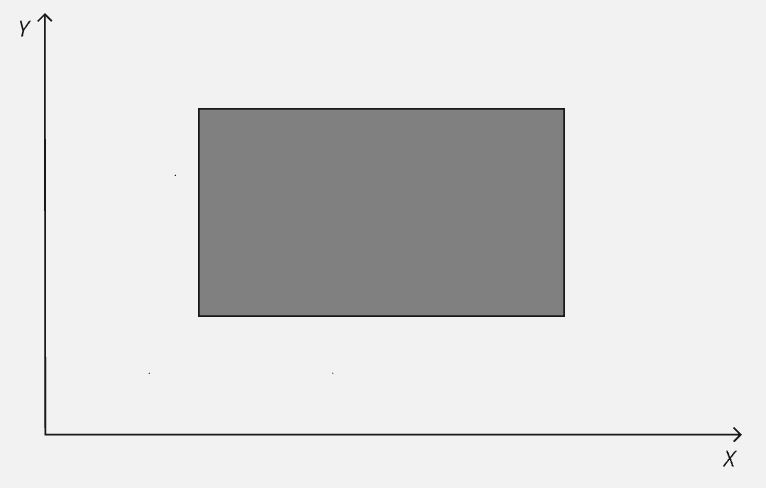
\includegraphics[width=\linewidth]{figures/Conceptos previos/Multi-intervalos/denso.png}
    \caption{Multi-intervalo denso — línea continua}
  \end{subfigure}
  \hfill
  \begin{subfigure}[b]{0.48\textwidth}
    \centering
    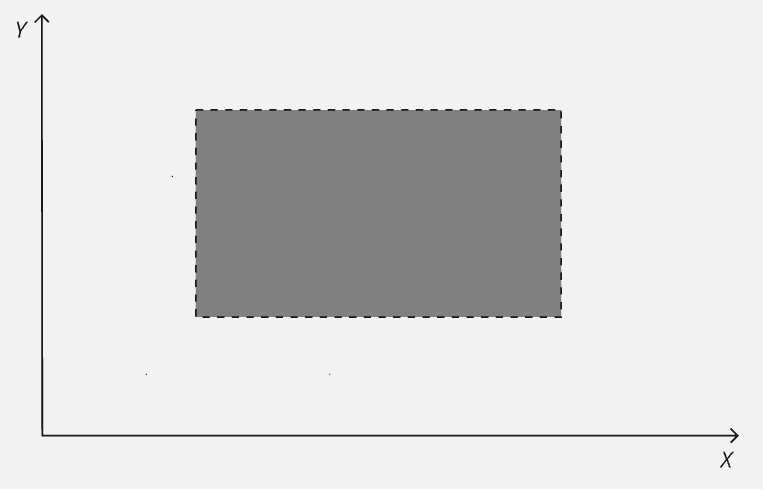
\includegraphics[width=\linewidth]{figures/Conceptos previos/Multi-intervalos/no-denso.png}
    \caption{Multi-intervalo no denso — línea discontinua}
  \end{subfigure}
  \caption{Representación de multi-intervalos bidimensionales}
  \label{fig:multiintervalos}
\end{figure}

Adicionalmente, se incluirá una representación gráfica que resalta el elemento mínimo y máximo de un multi-intervalo. Para ello, se utilizará un punto verde para indicar el mínimo y un punto rojo para el máximo. En la Figura~\ref{fig:multi} se muestra esta representación de manera ilustrativa.

\begin{figure}[ht]
  \centering
  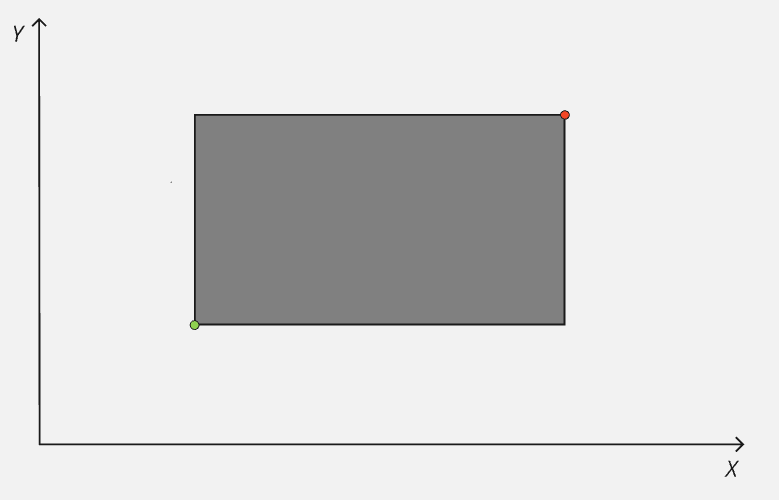
\includegraphics[width=0.6\textwidth]{figures/Conceptos previos/Multi-intervalos/minmax.png}
  \caption{Representación de un multi-intervalo con su mínimo (verde) y máximo (rojo).}
  \label{fig:multi}
\end{figure}


\section{Conjuntos}

\begin{center}
    \textit{Se modela un conjunto como una familia o colección de multi-intervalos no vacíos de igual cantidad de dimensiones y disjuntos dos a dos, es decir, no comparten ningún valor multi-dimensional d entre ellos.}
\end{center}

En consecuencia, la dimensión de un conjunto no está determinada por la cantidad total de multi-intervalos que lo componen, sino que corresponde a la dimensión de cualquiera de ellos.

La notación que se le dará a los conjuntos será la siguiente:

\begin{center}


    $\{i_{00} \times i_{01} \ \ldots \ \times i_{0(k-1)},\ i_{10} \times i_{11} \ \ldots \ \times i_{1(k-1)}\, \ldots,\ i_{(i-1)0} \times i_{(i-1)1} \ \ldots \ \times i_{(i-1)(k-1)}\}$
    
    Omitiendo los multi-intervalos:
    
    $\{mdi_0,\ mdi_1\ \ldots,\ mdi_{i-1}\}$

    donde $i$ es la cantidad de multi-intervalos del conjunto y $k$ es la cantidad de dimensiones que tendrán los mismos.
\end{center}

En particular, el conjunto vacío se representará de la siguiente manera: $\{\}$. Y en particular se utilizara la notación $\kappa(A)$ para representar la cantidad de multi-intervalos del conjunto $A$.


En primera instancia se verán todas las funciones relevantes que los conjuntos tienen disponibles en términos generales, ya que en el proyecto se disponen de múltiples implementaciones de conjuntos.

\subsection{Conjuntos generales}


La estructura \texttt{SetDelegate} representa un tipo base abstracto que define una interfaz común para manipulación de conjuntos de multi-intervalos. Este tipo se define como parte del conocido patrón de diseño \textit{delegate}, utilizado en este contexto para encapsular distintas implementaciones concretas de conjuntos dentro de una estructura delegadora. Esta estructura delegadora corresponde al tipo \texttt{Set}. De este modo, siempre que se requiera trabajar con conjuntos fuera de su implementación, se empleará una instancia de \texttt{Set}, la cual contendrá una implementación concreta de conjuntos del tipo \texttt{SetDelegate}.


Entre estas implementaciones concretas se encuentran: \texttt{UnorderedSet}, que representa conjuntos desordenados; y \texttt{OrderedDenseSet}, que modela conjuntos ordenados densos, es decir, con una única dimensión y con paso igual a uno. A partir de aquí.


Se han definido las siguientes operaciones sobre los conjuntos en la interfaz propuesta por \texttt{SetDelegate} :

\begin{itemize}
    \begin{comment}
    
    %sacable
    \item \texttt{SetDelegate() (Sin argumentos):}  
    Crea un conjunto vacío, es decir, $\{\}$.
    %sacable
    \item \texttt{SetDelegate(const MD\_NAT \&x):}  
    Crea un conjunto con un único multi-intervalo utilizando a $x$.
%sacable
    \item \texttt{SetDelegate(const Interval \&i):}  
    Crea un conjunto con un único multi-intervalo que solo contiene a $i$.
%sacable
    \item \texttt{SetDelegate(const SetPiece \&mdi):}  
     Crea un conjunto con un único multi-intervalo $mdi$.
    \end{comment}

    \item \texttt{virtual bool operator==(const SetDelegate \&other) const = 0:}  
    Verifica que los dos conjuntos tengan exactamente los mismos elementos.

    \begin{center}
        \textbf{Por ejemplo:} $\{[0: 1: 10] \times [11: 1: 20] \times [21: 1: 21]\}\texttt{==}\{[0: 1: 10] \times [11: 1: 20] \times [21: 1: 21]\}=\texttt{true}$.
    \end{center}

    \item \texttt{virtual bool operator!=(const SetDelegate \&other) const = 0:}  
    Verifica que los dos conjuntos no ten

    \begin{center}
        \textbf{Por ejemplo:} $\{[0: 1: 10] \times [11: 1: 20] \times [21: 1: 21]\}\texttt{!=}\{\}=\texttt{true}$.
    \end{center}

    \item \texttt{virtual std::size\_t size() const = 0:}
     Devuelve la cantidad de multi-intervalos en el conjunto.

    \begin{center}
        \textbf{Por ejemplo:} $size(\{[0: 1: 10] \times [11: 1: 20] \times [21: 1: 21]\})=1$.
    \end{center}
     
     \item \texttt{virtual void emplaceBack(const SetPiece \&mdi) = 0:}
     Agrega un multi-intervalo $mdi$ más al final del conjunto.

    \begin{center}
        \textbf{Por ejemplo:} $emplaceBack(\{[0: 1: 10] \times [11: 1: 20] \times [21: 1: 21]\}, [11: 1: 21] \times [11: 1: 20] \times [21: 1: 21])=\{[0: 1: 10] \times [11: 1: 20] \times [21: 1: 21], [11: 1: 21] \times [11: 1: 20] \times [21: 1: 21]\}$.
    \end{center}

     \item \texttt{virtual void emplace(const SetPiece \&mdi) = 0:}
     Agrega un multi-intervalo $mdi$ en algún lugar, donde corresponda, del conjunto.

     \begin{center}
        \textbf{Por ejemplo:} $emplace(\{[0: 1: 10] \times [11: 1: 20] \times [21: 1: 21]\},$
        
        $ [11: 1: 21] \times [11: 1: 20] \times [21: 1: 21])=$
        
        $\{[0: 1: 10] \times [11: 1: 20] \times [21: 1: 21], [11: 1: 21] \times [11: 1: 20] \times [21: 1: 21]\}$.
    \end{center}
    
    \item \texttt{virtual unsigned int cardinal() const = 0:}  
    Devuelve la cantidad de elementos contenidos en el conjunto. En escancia la suma del cardinal de todos los multi-intervalos que lo conforman.

     \begin{center}
        \textbf{Por ejemplo:} $cardinal(\{[0: 1: 10]\})=11$.
    \end{center}

    \item \texttt{virtual bool isEmpty() const = 0:}  
    Verifica si un conjunto es vacío, es decir, no contiene multi-intervalos.

         \begin{center}
        \textbf{Por ejemplo:} $isEmpty(\{[0: 1: 10]\})=\texttt{false}$.
    \end{center}

    \item \texttt{virtual MD\_NAT minElem() const = 0:}  
    Devuelve el mínimo elemento del conjunto.

    \begin{center}
        \textbf{Por ejemplo:} $minElem(\{[0: 1: 10], [15: 1: 100]\})=0$.
    \end{center}

    \item \texttt{virtual MD\_NAT maxElem() const = 0:}  
    Devuelve el máximo elemento del conjunto.

    \begin{center}
        \textbf{Por ejemplo:} $maxElem(\{[0: 1: 10], [15: 1: 100]\})= 100$.
    \end{center}

    \item \texttt{virtual SetDelegPtr intersection(const SetDelegate \&other) const = 0):}  
    Realiza la intersección entre el conjunto que invoca el método y el conjunto $other$. Si estos no tienen elementos en común, devuelve el conjunto vació.

    \begin{center}
        \textbf{Por ejemplo:} $intersection(\{[0: 1: 100], [500: 1: 1000]\},\{[1000: 1: 10000]\})= \{[1000: 1: 1000]\}$.
    \end{center}

    \item \texttt{virtual SetDelegPtr cup(const SetDelegate \&other) const = 0:}  
    Realiza la union entre el conjunto que invoca el método y el conjunto $other$.

    \begin{center}
        \textbf{Por ejemplo:} $cup(\{[0: 1: 100], [500: 1: 1000]\},\{[500: 1: 1000],[1400: 1: 10000]\})=$
        
        $ \{[0: 1: 100],[500: 1: 1000],[1400: 1: 10000]\}$.
    \end{center}

    \item \texttt{virtual SetDelegPtr complement() const = 0:}  
    Obtiene el complemento del conjunto que invoca el método.

    
    \begin{center}
        \textbf{Por ejemplo:} $complement(\{[10: 1: 100]\})= \{[0: 1: 9],[101: 1: \texttt{Inf}]\}$.
    \end{center}

    \item \texttt{virtual SetDelegPtr difference(const SetDelegate \&other) const = 0:}  
    Realiza la diferencia entre el conjunto que invoca el método y el conjunto $other$, es decir, al invocante se le resta $other$.

    \begin{center}
        \textbf{Por ejemplo:} $difference(\{[1: 1: 2], [3: 1: 100]\},\{[50: 1: 100]\})= \{[1: 1: 2], [3: 1: 49]\}$.
    \end{center}
    
        
    \item \texttt{virtual std::size\_t arity() const = 0}:  
    Devuelve la cantidad de dimensiones que tiene el conjunto, es decir, la aridad de los multi-intervalos que lo componen.

    \begin{center}
        \textbf{Por ejemplo:} $arity(\{[0: 1: 10] \times [11: 1: 20] \times [21: 1: 21]\})=3$.
    \end{center}
    
    \item \texttt{virtual SetDelegPtr disjointCup(const SetDelegate \&other) const = 0:}  
    Realiza la unión disjunta entre el conjunto que invoca el método y el conjunto $other$. Se asume que los argumentos son conjuntos disjuntos.

    \begin{center}
        \textbf{Por ejemplo:} $disjointCup(\{[1: 1: 2], [3: 1: 100]\},\{[0: 1: 0],[1000: 1: 3000]\})=\{[1: 1: 2],$
        
        $ [3: 1: 100],[0: 1: 0],[1000: 1: 3000]\}$.
    \end{center}
    
    \begin{comment}
%sacable
    \item \texttt{virtual SetDelegPtr filterSet(bool (*f)(const SetPiece \&mdi)) const = 0:}  
    Devuelve un conjunto con aquellos multi-intervalos que hayan pasado el predicado $f$.
%sacable
    \item \texttt{virtual SetDelegPtr offset(const MD\_NAT \&off) const = 0:}  
    Devuelve un conjunto con todos los elementos del conjunto que invoco al método desplazados un offset $off$, es decir, se le aplica el método offset con $off$ a cada multi-intervalo.
    \end{comment}
    \item \texttt{virtual SetDelegPtr compact() const = 0:}  
    Devuelve el conjunto resultante de intentar compactar los distintos multi-intervalos del conjunto que invoca el método con el resto de los multi-intervalos.

    \begin{center}
        \textbf{Por ejemplo:} $compact(\{[0: 1: 10] \times [11: 1: 20] \times [21: 1: 21]\})= \{[0: 1: 21]\}$.
    \end{center}

\end{itemize}


Para cumplir con el objetivo de proporcionar una implementación concreta de conjuntos ordenados, se decidió tomar como punto de partida la implementación ya existente de conjuntos desordenados. 

Aunque, como se indicó anteriormente, no es el propósito de este documento detallar dichas implementaciones previas, se explicará con mayor profundidad el funcionamiento de la operación \texttt{complement} en el caso de conjuntos desordenados, ya que se considera útil especialmente para facilitar y modularizar la comprensión de las optimizaciones propuestas.


Asimismo, se incluirá una descripción más breve de otras operaciones relevantes, tales como \texttt{intersection} y \texttt{disjointCup}.

\subsection{Conjuntos desordenados}\label{sec:conjs-des}

Cabe destacar que la estructura \texttt{UnorderedSet} se encuentra compuesta exclusivamente por una colección de multi-intervalos, almacenada en una variable denominada \texttt{pieces\_}. Esta colección se implementa mediante un contenedor de tipo \texttt{vector<SetPiece>}.

\textbf{Pseudocódigo/Notación:} En este capítulo los diferentes multi-intervalos de un conjunto desordenado se indexarán mediante subíndices. En particular, $A_i$ representará el $i$-ésimo multi-intervalo del conjunto desordenado $A$, lo cual corresponde a \texttt{pieces\_[i]} en C++, con $i \in \{0, \ldots, \kappa(A)-1\}$.

\subsubsection{Intersección - \texttt{intersection}}

Como se puede observar en el Algoritmo~\ref{alg:interseccionDes} el pseudocódigo para la operación \texttt{intersection}, la implementación de la intersección entre conjuntos desordenados resulta, en esencia, relativamente simple y directa, si se excluyen los casos especiales que optimizan su ejecución. 

El enfoque central de esta operación consiste en iterar sobre todos los multi-intervalos que conforman el conjunto desordenado $A$ y, para cada uno de ellos, computar su intersección con todos los multi-intervalos del conjunto desordenado $B$. De esta forma, se construye un nuevo conjunto cuyos elementos corresponden a las intersecciones no vacías entre los pares de multi-intervalos provenientes de $A$ y $B$ respectivamente.

\begin{algorithm}
\caption{Intersección entre conjuntos desordenados}\label{alg:interseccionDes}
\begin{algorithmic}[1]
\Require $A$, $B$ son conjuntos desordenados
\Ensure $C$ es un conjunto desordenado que representa $A \cap B$
\Function{intersection}{$A, B$}

\State $C := \{\}$

\If{$\Call{isEmpty}{A}$ \textbf{or} $\Call{isEmpty}{B}$}
    \State \Return $C$
\EndIf

\If{$\Call{maxElem}{A} < \Call{minElem}{B}$ \textbf{or} $\Call{maxElem}{B} < \Call{minElem}{A}$}
    \State \Return $C$
\EndIf

\If{$\Call{maxElem}{A} == \Call{minElem}{B}$}
    \State $C := \{ \Call{maxElem}{A} \}$
    \State \Return $C$
\EndIf

\If{$\Call{maxElem}{B} == \Call{minElem}{A}$}
    \State $C := \{\Call{minElem}{A} \}$
    \State \Return $C$
\EndIf

\If{$A == B$}
    \State \Return $A$
\EndIf

\

\ForAll{$a \in A$}
    \ForAll{$b \in B$}
        \State $mdi := \Call{intersection}{a,b}$
        \If{$i \neq \emptyset$}
            \State $\Call{emplaceBack}{C,mdi}$
        \EndIf
    \EndFor
\EndFor

\State \Return $C$
\EndFunction
\end{algorithmic}
\end{algorithm}

\subsubsection{Complemento - \texttt{complement}}

El cálculo del complemento de conjuntos desordenados se define a partir de dos funciones principales: \texttt{complement} y \texttt{complementAtom}. 

La función \texttt{complement} es la encargada de realizar el cálculo general del complemento para un conjunto arbitrario con ayuda de la operación \texttt{intersection}, mientras que \texttt{complementAtom} se especializa en calcular el complemento de un conjunto que contiene únicamente un multi-intervalo.

A continuación, se detalla el funcionamiento específico de ambas funciones.


\textbf{Complement}

La operación de complemento, denominada \texttt{complement}, permite calcular el complemento de un conjunto desordenado compuesto por una cantidad variable de multi-intervalos. En el pseudocódigo, Algoritmo~\ref{alg:complementDes}, se presenta la operación \texttt{complement}, donde se ilustra su funcionamiento.  

Desde una perspectiva teórica de conjuntos, la operación busca calcular la siguiente expresión:

\[
\bigcap_{i=0}^{ \kappa(A)-1} \overline{\{A_i\}}
\]

La cual se fundamenta en que:

\[
A = \{A_0, A_1, A_2, \ldots, A_{\kappa(A)-1}\} 
    = \bigcup_{i=0}^{\kappa(A)-1} \{A_i\}
\]

y, por lo tanto,

\[
\overline{A} 
    = \overline{\bigcup_{i=0}^{\kappa(A)-1} \{A_i\}}
    = \bigcap_{i=0}^{\kappa(A)-1} \overline{\{A_i\}}.
\]



\begin{comment}
Aquí se describe la operación principal que permite calcular el complemento de un conjunto desordenado con una cantidad variable de multi-intervalos, \texttt{complement}. Seguidamente, se presenta el pseudocódigo de la operación ~\ref{alg:complementDes}, junto con el procedimiento que se lleva a cabo:



\begin{enumerate}
    \item En primer lugar, se calcula el complemento de un conjunto atómico compuesto únicamente por el primer multi-intervalo del conjunto $A$, utilizando la función \textit{complementAtom} y guardándolo como resultado final en $C$. Esta función será explicada más adelante; por ahora, basta con saber que genera un conjunto desordenado que representa el complemento de un conjunto formado por un único multi-intervalo.
    
    \item Luego, se calcula el \textit{complementAtom} del siguiente multi-intervalo del conjunto $A$, en caso de que exista, y se realiza la intersección entre el resultado actual $C$ y el conjunto complemento resultante de dicho multi-intervalo.
    
    \item Finalmente, se guarda el resultado de la intersección y se repite desde el paso anterior hasta que no queden más multi-intervalos por recorrer en $A$. Posteriormente se devuelve $C$, que es el complemento de $A$.
\end{enumerate}

\end{comment}



\begin{algorithm}
\caption{Complemento de un conjunto desordenado}\label{alg:complementDes}
\begin{algorithmic}[1]
\Require $A$ es un conjunto desordenado 
\Ensure $C$ es un conjunto desordenado que representa el complemento de $A$
\Function{complement}{$A$}
\State $C := \{\}$
\State $first\_mdi := A_0$
\State $C :=$  \Call{complementAtom}{$first\_mdi$} 
\For{$i := 1$; $i\neq size(A)$; $i$\!+\!+}
    \State $mdi := A_i$
    \State $atomic\_set :=$ \Call{complementAtom}{$mdi$}
    \State $C :=$ \Call{intersection}{$C$,$atomic\_set$}
\EndFor
\State \textbf{return} $C$
\EndFunction
\end{algorithmic}
\end{algorithm}



En la Figura~\ref{fig:complemento} se muestra gráficamente cómo se va calculando el complemento de un conjunto desordenado. En particular en este ejemplo el conjunto $A$ tiene solo multi-intervalos densos. Se eligieron multi-intervalos densos para que la representación gráfica sea mas sencilla de comprender.

\begin{figure}[H]
    \centering
    
    % Imagen principal grande
    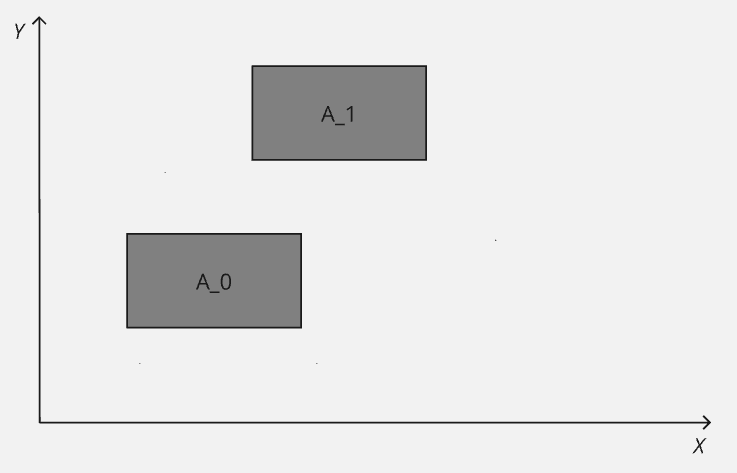
\includegraphics[width=0.6\textwidth]{figures/Conceptos previos/Conjuntos/conjuntoAcomp.png}
    \caption*{(a) Conjunto desordenado $A$}
    
    \vspace{1em}
    
    % Subfiguras en 3 columnas (6 imágenes en total)
    \begin{minipage}{0.31\textwidth}
        \centering
        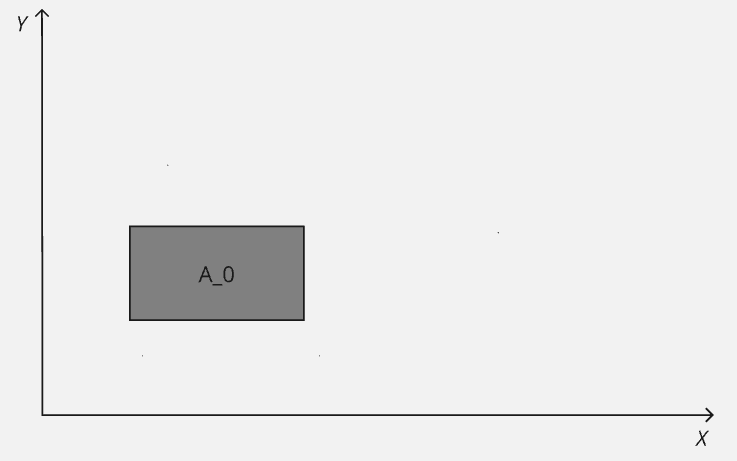
\includegraphics[width=\textwidth]{figures/Conceptos previos/Conjuntos/iter1comp.png}
        \caption*{    \centering (b1) Conjunto atómico con $A_0$}
    \end{minipage}
    \begin{minipage}{0.31\textwidth}
        \centering
        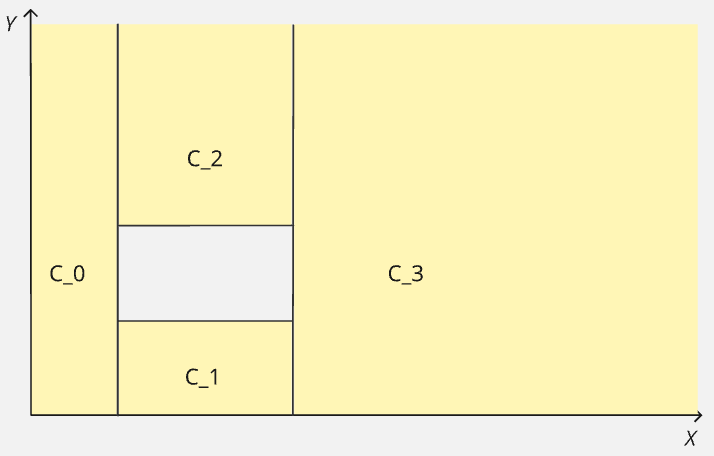
\includegraphics[width=\textwidth]{figures/Conceptos previos/Conjuntos/iter1compA.png}
        
        \caption*{     \centering (b2) Complemento del conjunto atómico}
    \end{minipage}
    \begin{minipage}{0.31\textwidth}
        \centering
        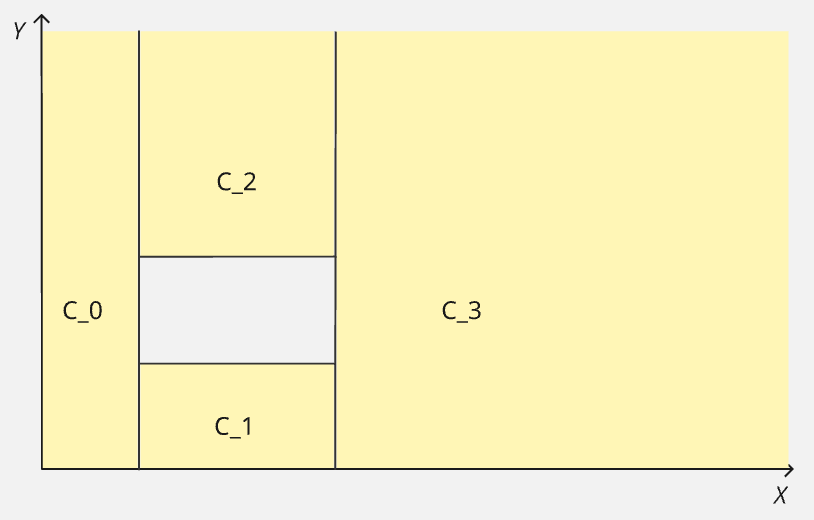
\includegraphics[width=\textwidth]{figures/Conceptos previos/Conjuntos/C1comp.png}
        \caption*{    \centering (b3) Conjunto $C$}
    \end{minipage}
    
    \vspace{1em}
    
    \begin{minipage}{0.31\textwidth}
        \centering
        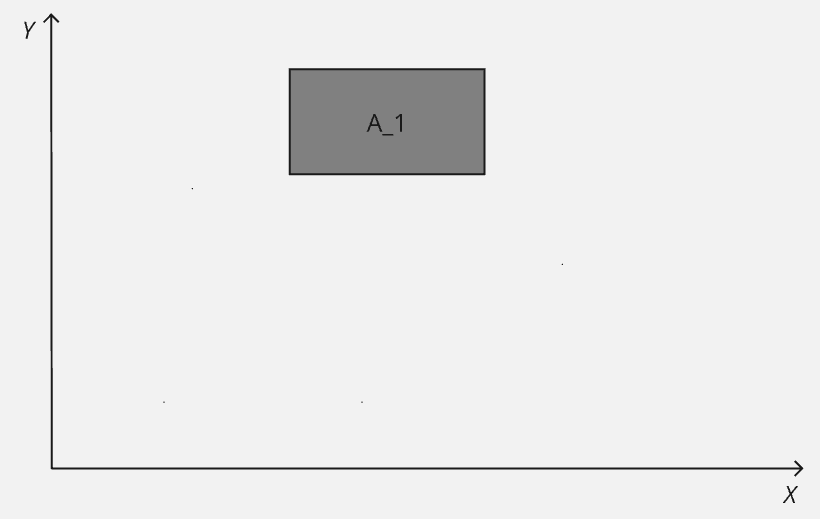
\includegraphics[width=\textwidth]{figures/Conceptos previos/Conjuntos/iter2comp.png}
        \caption*{    \centering (b4) Conjunto atómico con $A_1$}
    \end{minipage}
    \begin{minipage}{0.31\textwidth}
        \centering
        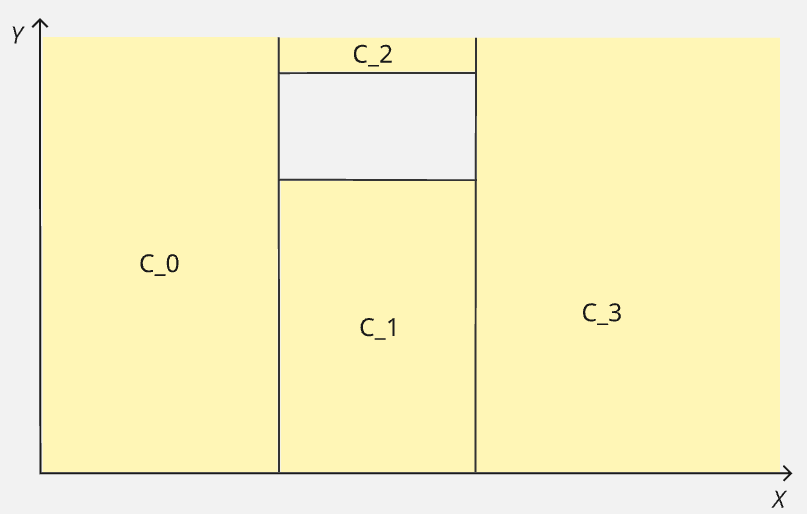
\includegraphics[width=\textwidth]{figures/Conceptos previos/Conjuntos/iter2compA.png}
        \caption*{    \centering (b5) Complemento del conjunto atómico}
    \end{minipage}
    \begin{minipage}{0.31\textwidth}
        \centering
        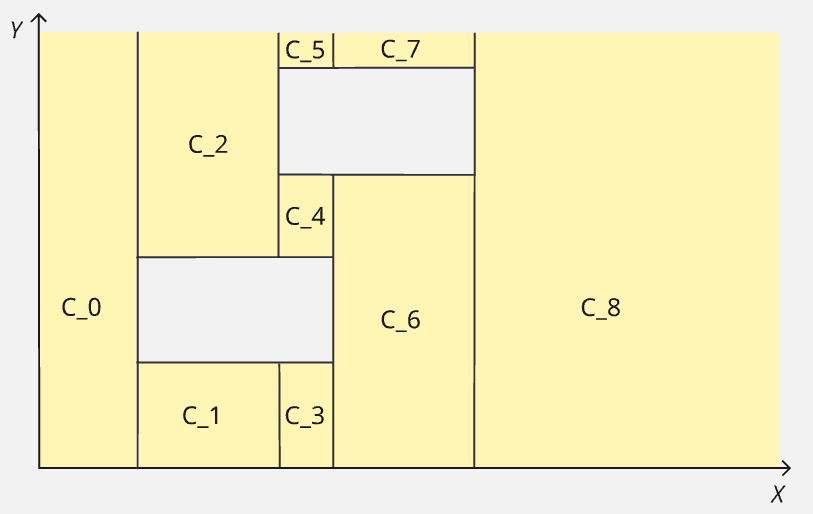
\includegraphics[width=\textwidth]{figures/Conceptos previos/Conjuntos/C2comp.png}
        \caption*{    \centering (b6) Conjunto $C$}
    \end{minipage}
    
    \caption{Visualización del cálculo del complemento de un conjunto desordenado con multi-intervalos densos $A$.}
    \label{fig:complemento}
\end{figure}


\textbf{ComplementAtom}

Una vez descrita la operación \texttt{complement} de conjuntos desordenados, lo único que resta por detallar es cómo se calcula el complemento de un conjunto desordenado que contiene un único multi-intervalo. Esta tarea es realizada por la operación \textit{complementAtom}.  
El procedimiento que dicha operación lleva a cabo se encuentra plasmado en el pseudocódigo de la operación en el Algoritmo~\ref{alg:ComplementAtomDes}, y puede explicarse de la siguiente manera:

\begin{enumerate}
    \item Se inicia el proceso con tres multi-intervalos fundamentales: $dense\_mdi$, que tiene la misma disposición de intervalos que el del conjunto original, pero con paso 1 en todos ellos(representando al multi-intervalo en su versión completamente densa); $during\_mdi$, que inicialmente es una copia de $dense\_mdi$ y $all$, que representa el multi-intervalo universo, con la misma aridad que el multi-intervalo del conjunto.

  \item Ahora bien, para calcular el complemento del conjunto atómico, se tendrán que recorrer una a una las dimensiones del multi-intervalo interno con la siguiente lógica:
  \begin{enumerate}
    \item \textbf{Selección de la dimensión.}  
      Se empieza por la dimensión \(d=0\). Y se extrae en base a ella el intervalo original del multi-intervalo del cual se quiere obtener el complemento: 
      \[
        d = [d_{\mathrm{begin}}:d_{\mathrm{step}}:d_{\mathrm{end}}].
      \]
    \item \textbf{Región “antes” del intervalo.}  
      Si \(d_{\mathrm{begin}}>0\), existe un rango no cubierto entre \(0\) y \(d_{\mathrm{begin}}-1\). Entonces se toma el multi-intervalo universo \(\mathit{all}\) y se lo restringe en la dimensión \(d\) a  
      \[
        [0:1:d_{\mathrm{begin}}-1].
      \]
      dejando los intervalos de las demás dimensiones sin cambios. Esa variación de \(\mathit{all}\) se añade al conjunto parcial de resultados $C$ y luego deshace el cambio.
    \item \textbf{Huecos “durante” el intervalo.}  
      Si el paso \(d_{\mathrm{step}}>1\), el intervalo original salta posiciones; entre cada salto quedan “huecos” que también forman parte del complemento. Para cada \(j=0,\dots,d_{\mathrm{step}}-2\) construimos  
      \[
        [d_{\mathrm{begin}}+j+1:d_{\mathrm{step}}:d_{\mathrm{end}}],
      \]
      y lo insertamos en una copia de nuestro multi-intervalo base, $during\_mdi$, y lo metemos en el conjunto desordenado resultante $C$.
      
    \item \textbf{Región “después” del intervalo.}  
      Si \(d_{\mathrm{end}}<\ \texttt{Inf}\), hay un rango desde \(d_{\mathrm{end}}+1\) hasta \texttt{Inf} de valores no abarcados por $i$. De nuevo se usa \(\mathit{all}\) restringido en \(d\) a  
      \[
        [i_{\mathrm{end}}+1:1: \texttt{Inf}],
      \]
       se lo añade al conjunto de resultados y se revierte el cambio de $all$.
    \item \textbf{Restauración y avance.}  
      Tras procesar el “antes”, “durante” y “después” en la dimensión \(d\), se actualizan \(\mathit{all}\) y $during\_mdi$, colocándoles los valores densos y originales de la dimensión \(d\) del multi-intervalo del cual estamos sacando el complemento respectivamente. Luego se pasa a la siguiente dimensión \(d+1\), y se repite todo el procedimiento.
  \end{enumerate}
\end{enumerate}

En la Figura a siguiente se muestra gráficamente cómo se va calculando el complemento atómico de un conjunto desordenado con un único multi-intervalo. En particular en este ejemplo el conjunto tiene un solo multi-intervalo no denso.
 
\begin{figure}[H]
    \centering
    
    % Imagen principal grande
    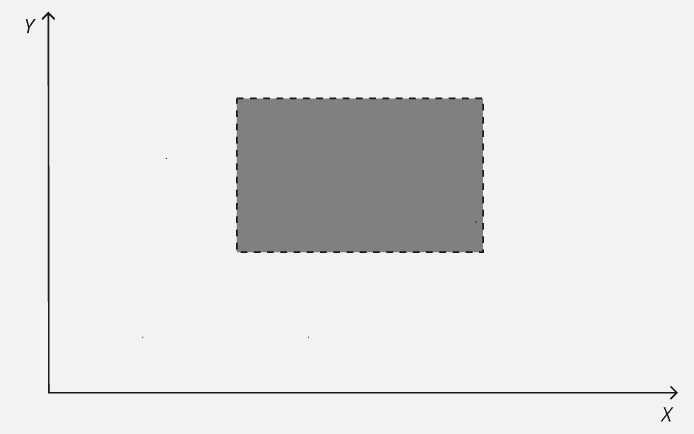
\includegraphics[width=0.6\textwidth]{figures/Conceptos previos/Conjuntos/compAtom1.png}
    \caption*{(a) Conjunto desordenado atómico}
    
    \vspace{1em}
    \begin{minipage}{0.41\textwidth}
        \centering
        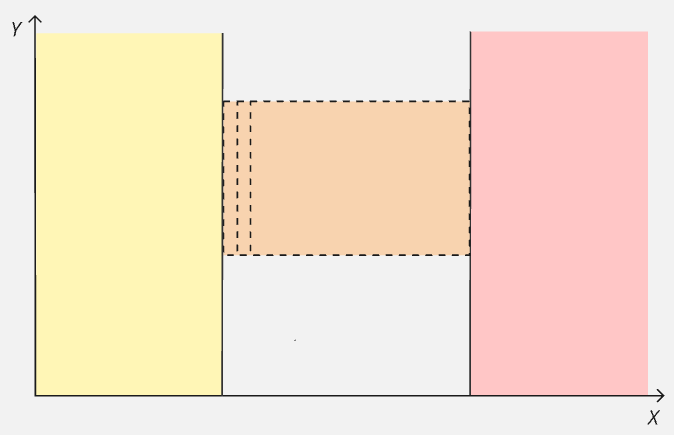
\includegraphics[width=\textwidth]{figures/Conceptos previos/Conjuntos/compAtom2.png}
        
        \caption*{     \centering (b1) Multi-intervalos resultantes del complemento atómico sobre la primera dimensión $x$}
    \end{minipage}
    \begin{minipage}{0.41\textwidth}
        \centering
        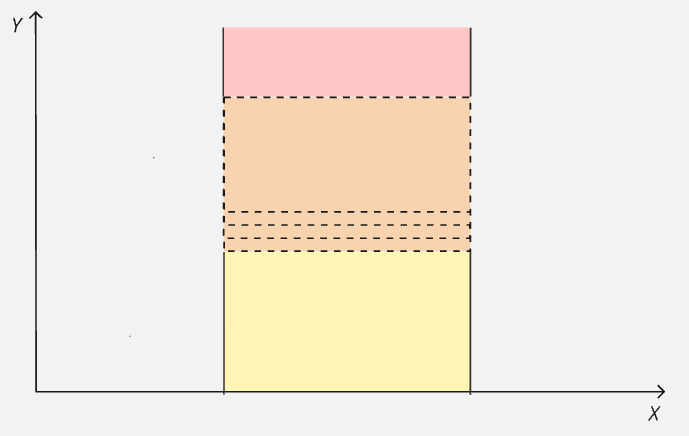
\includegraphics[width=\textwidth]{figures/Conceptos previos/Conjuntos/compAtom3.png}
        \caption*{    \centering (b2) Multi-intervalos resultantes del complemento atómico sobre la segunda dimensión $y$}
    \end{minipage}
    
    \caption{Visualización del cálculo del complemento atómico sobre un conjunto desordenado atómico no denso.}
    \label{fig:complemento}
\end{figure}

\begin{algorithm}
\caption{Complemento atómico de conjunto ordenado atómico}
\label{alg:ComplementAtomDes}
\begin{algorithmic}[1]
\Require $A$ es un conjunto ordenado atómico
\Ensure Un conjunto desordenado $C$, el complemento de $A$
\Function{complementAtom}{$A$}
  \State $C := \emptyset$  
  \State $mdi := A_0$  
  \State $dense\_mdi := ||$
  \ForAll{$interval \in mdi$}
    \State $i := $$[$\Call{begin}{$interval$} $:1:$ \Call{end}{$interval$}$]$
    \State \Call{emplaceBack}{$dense\_mdi,i$}
  \EndFor

  \State $during\_mdi := dense\_mdi$
  \State $univ := [0:1:\texttt{Inf}]$
  \State $all := |univ|^{\Call{arity}{A}}$ \Comment{Representa el universo completo de aridad $\Call{arity}{A}$}

  \State $dim := 0$
  \ForAll{$i \in mdi$}

    \If{\Call{begin}{$i$} $\neq 0$}
      \State $i\_res := [0:1:$ \Call{begin}{$i$}$-1]$
      \If{$\neg \Call{isEmpty}{i\_res}$}
        \State $all[dim] := i\_res$
        \State $C := C \frown \{all\}$
        \State $all[dim] := univ$
      \EndIf
    \EndIf

    \If{\Call{begin}{$i$} $<$ \texttt{Inf}}
        \If{\Call{step}{$i$} $> 1$}
          \For{$j = 0$; $i < size(A)$; $j$\!+\!+}
            \State $h := [$\Call{begin}{$i$}$ + j + 1 : $\Call{step}{$i$} $: $ \Call{end}{$i$}$]$
            \If{$\neg \Call{isEmpty}{h}$}
              \State $during\_mdi[dim] := h$
              \State $C := C \frown during\_mdi$
            \EndIf
          \EndFor
        \EndIf
    \EndIf

    \If{\Call{end}{$i$} $<$ \texttt{Inf}}
      \State $i\_res := [$\Call{end}{$i$}$+1 : 1 : \texttt{Inf}]$
      \If{$\neg \Call{isEmpty}{i\_res}$}
        \State $all[dim] := i\_res$
        \State $C := C \frown \{all\}$
        \State $all[dim] := univ$
      \EndIf
    \EndIf

    \State $all[dim] := dense\_mdi[dim]$
    \State $during\_mdi[dim] := i$
    \State $dim \!+\!+$
  \EndFor
  \State \Return $C$
\EndFunction
\end{algorithmic}
\end{algorithm}


\begin{comment}
\subsubsection{Diferencia - \texttt{defference}}

Al igual que ocurre con la operación de unión (la cual será abordada más adelante), la disponibilidad previa de las operaciones de intersección y complemento permite implementar la diferencia de conjuntos desordenados de manera sencilla. Esta estrategia modular se refleja claramente en la simplicidad de la función \texttt{difference}, cuyo pseudocódigo se presenta en ~\ref{alg:differenceDes} y que constituye precisamente la operación encargada de calcular la diferencia entre conjuntos desordenados.


\begin{algorithm}
\caption{Diferencia de conjuntos desordenados}\label{alg:differenceDes}
\begin{algorithmic}[1]
\Require $A$, $B$ son conjuntos desordenados
\Ensure $C$ es el conjunto $A \setminus B$
\Function{difference}{$A$, $B$}

\If{$A == \emptyset$ \textbf{or} $B == \emptyset$}
    \State \textbf{return} $A$
\EndIf

\State $B' :=$ \Call{complement}{$B$}
\State $C:=$ \Call{intersection}{$A$, $B'$}

\State \textbf{return} $C$
\EndFunction
\end{algorithmic}
\end{algorithm}

    
\end{comment}


\subsubsection{Unión disjunta - \texttt{disjointCup}}

En lo que respecta a la operación correspondiente a la \textit{unión disjunta}(\texttt{disjointCup}), al igual que la intersección, se trata de una operación conceptualmente sencilla. Esta simplicidad se ve reflejada en el pseudocódigo del Algoritmo~\ref{alg:disjointcupDes}. Dado que los conjuntos involucrados son desordenados y, por hipótesis, disjuntos entre sí, la operación no requiere verificaciones adicionales de solapamiento o duplicación de elementos. Basta simplemente con reunir todos los multi-intervalos de ambos conjuntos en una único conjunto desordenado para obtener el resultado deseado.


\begin{algorithm}
\caption{Unión disjunta de dos conjuntos desordenados}\label{alg:disjointcupDes}
\begin{algorithmic}[1]
\Require $A$, $B$ son conjuntos desordenados
\Ensure $R$ es un conjunto desordenado que representa la unión disjunta de $A$ y $B$
\Function{disjointCup}{$A, B$}

\If{$\Call{isEmpty}{A}$}
  \State \Return $B$
\EndIf

\If{$\Call{isEmpty}{B}$ \textbf{or} $A == B$}
  \State \Return $A$
\EndIf

\State $R :=$ $A$
\ForAll{$b \in B$}
  \State $\Call{emplaceBack}{R,b}$
\EndFor

\State \Return $R$
\EndFunction
\end{algorithmic}
\end{algorithm}

\begin{comment}
\subsubsection{Unión - \texttt{cup}}

Como se explicó anteriormente, la operación de unión puede construirse a partir de operaciones ya disponibles, como lo son la diferencia y la unión disjunta. Esta reutilización de funciones básicas permite que el código de la unión resulte especialmente sencillo, ya que basta con aplicar las operaciones de conjuntos que, en conjuntos, son equivalentes a una unión de conjuntos. De esta manera, la implementación de la operación \texttt{cup} es particularmente compacta y clara.

\begin{algorithm}
\caption{Unión de conjuntos desordenados (\texttt{cup})}\label{alg:cup}
\begin{algorithmic}[1]
\Require $A$, $B$: conjuntos desordenados
\Ensure $R$: conjunto desordenado que representa la unión $A \cup B$
\Function{cup}{$A, B$}

\If{$A == \emptyset$}
  \State \Return $B$
\EndIf

\If{$B == \emptyset$  \textbf{or} $A == B$}
  \State \Return $A$
\EndIf

\If{$\max(A) < \min(B)$}
  \State $R := A$
  \ForAll{$\text{mdi} \in B$}
    \State \Call{emplaceBack}{$B, mdi$}
  \EndFor
  \State \Return $R$
\EndIf

\If{$\max(B) < \min(A)$}
  \State $R := B$
  \ForAll{$\text{mdi} \in A$}
    \State \Call{emplaceBack}{$A, mdi$}
  \EndFor
  \State \Return $R$
\EndIf

\State $D :=$ \Call{difference}{$A, B$}
\State \Return \Call{disjointCup}{$B, D$}

\EndFunction
\end{algorithmic}
\end{algorithm}   
\end{comment}


\subsection{Conjuntos ordenados densos}\label{sec:conjs-ord-dense}

A continuación, se presenta una breve descripción de cómo los conjuntos ordenados densos organizan los multi-intervalos de manera interna. Esta explicación resulta relevante dado que, por razones de conveniencia, se ha adoptado el mismo criterio de orden para los multi-intervalos contenidos en un conjunto ordenado.

En particular, los conjuntos ordenados densos emplean una variable miembro llamada \texttt{pieces\_}, de tipo \texttt{MDIOrdSet}, que es un sinónimo de \texttt{vector<SetPiece>}. Esta estructura almacena los multi-intervalos, los cuales se ordenan utilizando la operación $<$ definida para los multi-intervalos (\texttt{SetPiece}).

Internamente, el operador $<$ entre multi-intervalos evalúa si el mínimo del primer multi-intervalo es menor que el del segundo. Dado que los mínimos son de naturales multi-dimensionales(\texttt{MD\_NAT}), esta comparación se realiza mediante el operador $<$ definido para \texttt{MD\_NAT}. En si, el operador $<$ definido para el tipo \texttt{MD\_NAT} compara componente por componente dos \texttt{MD\_NAT}, siguiendo el siguiente criterio que luego se aplica a los mínimos de los multi-intervalos: 

\begin{center}
Sea $x = (x_0, x_1, \dots, x_{n-1})$ y $y = (y_0, y_1, \dots, y_{n-1})$ dos elementos de tipo \texttt{MD\_NAT}. Se define que $x < y$ si y sólo si existe un índice $j \in \{0, \dots, {n-1}\}$ tal que se cumplen simultáneamente las siguientes condiciones:
\end{center}

\begin{itemize}
    \item $x_j < y_j$, es decir, en la componente $j$, $x$ es menor que $y$;
    \item Para todo $i$ tal que $0 \leq i < j$, se cumple que $x_i = y_i$.
\end{itemize}

Ahora bien al trabajar con multi-intervalos de solo una dimensión, este operador de menor queda relegado a solo ser el $<$ tradicional de los naturales. Por ende dados los siguientes multi-intervalos de una dimensión:

\begin{center}
    
    $mdi_1 = |[0:3:9]|$, con mínimo 0.
    
    $mdi_2 = |[4:1:10]|$, con mínimo 4.
    
    $mdi_3 = |[2:2:4]|$, con mínimo 2.
    
\end{center}

Se tiene que el conjunto ordenado denso queda tal que así:

\begin{center}
    $\{mdi_1,\ mdi_3,\ mdi_2\}$
\end{center}

ya que:

\begin{center}
    $0 < 2 < 4$
\end{center}

\subsection{\textit{Abstract factory} para conjuntos}

Adicionalmente, se incorpora el patrón de diseño \textit{abstract factory}, aplicado a la creación de instancias del tipo \texttt{SetDelegate}. Para ello, se define la clase abstracta \texttt{SetAF}, que actúa como una interfaz común para diferentes fábricas concretas, como \texttt{UnordAF}, para conjuntos desordenados y \texttt{OrdDenseAF}, para conjuntos ordenados densos, cada una responsable de construir conjuntos con una representación interna específica.

Esta abstracción cobra especial relevancia en la sección de mapas. Allí, la fábrica de mapas (\texttt{MapAF}) extiende a \texttt{SetAF}, y reutiliza internamente una fábrica concreta de conjuntos para construir tanto dominios como imágenes de los mapas.

\section{Mapas lineales}

\begin{center}
\textit{
Un mapa lineal puede entenderse como una asociación entre un conjunto de multi-intervalos y una colección de expresiones lineales. Formalmente, un mapa lineal de aridad \( j \in \mathbb{N}\) se define como:
\[
\mathit{map} = \{ \mathit{mdi}_0,\ \mathit{mdi}_2,\ \ldots,\ \mathit{mdi}_{k-1} \} \mapsto [e_0,\ e_2,\ \ldots,\ e_{j-1}]
\]
donde cada $mdi_l$ es un multi-intervalo de aridad \( j \), con $l$ entre 0 y $k$ y con $k \in \mathbb{N}$, y cada \( e_i \), con $i$ entre 0 y $j$, es una expresión lineal de la forma \( m*x + h \), con $m,h \in \mathbb{Q}$.}  

\textit{
El dominio del mapa está conformado multi-intervalos, $mdi$, y cada expresión \( e_i \) se evalúa sobre la \( i \)-ésima dimensión de dichos multi-intervalos. En otras palabras, el dominio de \( e_i \) está compuesto por la colección de todos los intervalos que aparecen en la dimensión \( i \) de cada $mdi$ presente en el dominio.
}
\end{center}

Este concepto de mapa lineal coincide con el de función multidimensional cabe recalcar. Para afianzar la idea, véanse ejemplos en una, dos y tres dimensiones:

\medskip

\textbf{Ejemplo 1. Unidimensional}
\[
\mathit{map} = \{[0,1,2],[5,1,7]\}\mapsto[x+1].
\]
Por ejemplo: \((1)\!\mapsto\![2]\) \((6)\!\mapsto\![7]\)

\medskip

\textbf{Ejemplo 2. Bidimensional}
\[
\mathit{map}=\{[0,1,1]\times[0,1,1],[3,1,4]\times[3,1,4]\}
\mapsto[x_0+2,\;2*x_1-1].
\]
Por ejemplo:
\((0,1)\!\mapsto\![2,1],\;(3,4)\!\mapsto\![5,7].\)

\medskip

\textbf{Ejemplo 3. Tridimensional}
\[\;
\mathit{map} = \{[0,1,1]\times[0,1,1]\times[0,1,1],
                 [2,1,3]\times[2,1,3]\times[2,1,3]\}
\mapsto[x_{0},\;x_{1}+1,\;2*x_{2}-1].
\]
Por ejemplo:
\[
(1,0,1)\;\mapsto\;[1,1,1],\quad
(3,2,3)\;\mapsto\;[3,3,5].
\]

La estructura \textbf{Map} se utilizara para representar a los mapas lineales y esta constituida por lo que sigue:

\begin{itemize}
  \item \texttt{dom} (de tipo \textbf{Set}): representa el dominio del mapa.
  \item \texttt{exp} (de tipo \textbf{Exp}): contiene la(s) expresión(es) lineal(es) asociada(s).
    \item \texttt{fact} (de tipo \textbf{SetAF}): contiene una fábrica concreta utilizada para construir cualquier tipo de conjunto relacionado con el mapa
\end{itemize}

Cabe destacar que el tipo \texttt{Exp} representará una colección de expresiones lineales, es un sinónimo para \texttt{vector<LExp>}, donde \texttt{LExp} es tipo de estructura que representa a una única expresión lineal.

A continuación se presentan las operaciones que tienen a disposición los mapas:

\begin{itemize}

   \begin{comment}
       
    \item \texttt{Map(const SetAF \&fact):}
    Crea un mapa vacío, $\{\{\}_{\langle fact\rangle} \mapsto []\}$, a través la fabrica concreta de conjuntos $fact$ como referencia para su dominio.
        
    \item \texttt{Map(const SetAF \&fact, MD\_NAT x, Exp exp):}
    Construye un mapa que contiene un único elemento $x$, una $n$-upla, en su dominio basado en la fabrica concreta de conjuntos $fact$, y cuyas expresiones lineales son $exp$.
    \begin{center}
        \textbf{Por Ejemplo:} con $x = (1,2)$ y $exp = [x_0 + 2,\; x_1 + 3]$, el mapa resultante es $\{\{|[1:1:1]\times[2:1:2]|\}_{\langle fact\rangle} \mapsto [x_0 + 2,\; x_1 + 3]$\}.
       
    \end{center}

    \item \texttt{Map(const SetAF \&fact, Interval i, LExp le):}
    Crea un mapa cuyo dominio es el conjunto, construido a través de $fact$, de elementos del intervalo $i$, y su expresión lineal es $le$.
    \begin{center}
        \textbf{Por Ejemplo:} con $i = [1:1:5]$ y $le = 2*x$, se crea el mapa $\{\{|[1:1:5]|\}_{\langle fact\rangle} \mapsto [2*x]\}$.
    \end{center}

    \item \texttt{Map(const SetAF \&fact, SetPiece mdi, Exp exp):}
    Construye un mapa definido sobre un conjunto construido a partir de la fabrica concreta de conjuntos $fact$, con unicamente el multi-intervalo $mdi$, y con expresión lineal $exp$.
    \begin{center}
        \textbf{Por Ejemplo:} con $mdi = |[1:1:3] \times [0:1:2]|$ y $exp = [x_0 + 2,\; x_1 +3]$, el mapa resultante es $\{|[1:1:3] \times [0:1:2]|\}_{\langle fact\rangle} \mapsto [x_0 + 2,\; x_1 + 3]\}$.
    \end{center}

    \item \texttt{Map(const SetAF \&fact, Set s, Exp exp):}
    Construye un mapa cuyo dominio es el conjunto $s$ y su ley de aplicación es $exp$.
   \end{comment} 

    \item \texttt{bool operator==(const Map \&other) const:} Verifica si dos mapas son iguales, es decir, si sus dominios y expresiones son idénticos, o si sus dominios e imágenes son iguales en caso de que sea un mapa con una único expresión.
    \begin{center}
        \textbf{Por Ejemplo:} $\{[1:1:3]\} \mapsto [x] \,\texttt{==}\, \{[1:1:3]\} \mapsto [x] =  \textit{true}$.
    \end{center}

    \item \texttt{bool operator!=(const Map \&other) const:} Verifica si dos mapas son distintos.
    \begin{center}
        \textbf{Por Ejemplo:} $\{[1:1:3]\} \mapsto [x] \,\texttt{==}\, \{[1:1:3]\} \mapsto [x+1] =  \textit{true}$.
    \end{center}

    \item \texttt{Map operator+(const Map \&other) const:} Suma dos mapas realizando la intersección de sus dominios y sumando sus expresiones.
    \begin{center}
        \textbf{Por Ejemplo:} $\{[1:1:3]\} \mapsto  [x] + \{|[2:1:4]|\} \mapsto [2*x] = \{[2:1:3]\} \mapsto [3*x]$.
    \end{center}


    \item \texttt{std::size\_t arity() const:} Devuelve la aridad del dominio del mapa.
    \begin{center}
        \textbf{Por Ejemplo:} $arity(\{[1:1:5] \times [0:1:2]\} \mapsto [x,x]) = 2$.
    \end{center}

    \item \texttt{bool isEmpty() const:} Devuelve \texttt{true} si el mapa no tiene elementos en su dominio.
    \begin{center}
        \textbf{Por Ejemplo:} $isEmpty(\{\} \mapsto [x]) = \texttt{true}$.
    \end{center}

    \item \texttt{Map restrict(const Set \&subdom) const:} Restringe el dominio del mapa en base $subdom$.
    \begin{center}
        \textbf{Por Ejemplo:} $restrict(\{[0:1:10]\} \mapsto [x],\{[5:1:8]\}) = \{[5:1:8]\} \mapsto [x]$.
    \end{center}

    \item \texttt{Set image() const:} Devuelve el conjunto imagen del mapa.
    \begin{center}
        \textbf{Por Ejemplo:} $image(\{[0:1:3]\} \mapsto [2*x]) = \{[0:2:6]\}$.
    \end{center}

    \item \texttt{Set image(const Set \&subdom) const:} Imagen del mapa restringido por $subdom$.
    \begin{center}
        \textbf{Por Ejemplo:} $image(\{[0:1:3]\} \mapsto [2*x],\{[1:1:1]\}) = \{[2:1:2]\}$.
    \end{center}

    \item \texttt{Set preImage(const Set \&subcodom) const:} Preimagen del subconjunto de la imagen $subcodom$.
    \begin{center}
        \textbf{Por Ejemplo:} $preImage(\{[0:1:3]\} \mapsto [2*x],\{[4:1:4]\}) = \{[2:1:2]\}$.
    \end{center}

    \item \texttt{Map composition(const Map \&other) const:} Composición de mapas.
    \begin{center}
        \textbf{Por Ejemplo:} $composition(\{[0:1:3]\} \mapsto [x+1],\{[0:1:3]\} \mapsto [2*x]) = \{[0:1:3]\} \mapsto [2*x+1]$.
    \end{center}

    \item \texttt{Map minInv() const:} Calcula la inversa o pseudo-inversa de un mapa.
    \begin{center}
                \textbf{Por Ejemplo:}$composition(\{[5:1:10]\} \mapsto [x+1]) = \{[6:1:11]\} \mapsto [x-1]$.
    \end{center}
\begin{comment}
    \item \texttt{bool isId() const:} Verifica si el mapa es identidad.
    \begin{center}
        \textbf{Por Ejemplo:} con el mapa $\{ \{|[0:1:3]|\} \mapsto [x+1]\}$ llamando a la función \texttt{isId}, devuelve \texttt{false}.
    \end{center}
\end{comment}

    \item \texttt{MaybeMap compact(const Map \&other) const:} Compacta dominios si tienen la misma ley.
    \begin{center}

        \textbf{Por Ejemplo:} $composition(\{[0:1:3]\} \mapsto [x],\{[4:1:5]\} \mapsto [x]) = \{[0:1:5]\} \mapsto [x]$.

    \end{center}

\end{itemize}

Nuevamente, si se desea consultar todo el código relacionado con mapas, este se encuentra disponible en la carpeta \textit{sbg} del repositorio, específicamente en los archivos \textit{map.cpp} y \textit{map.hpp}.

\subsection{\textit{Abstract factory} de mapas}

En este caso, el patrón \textit{abstract factory} se aplica nuevamente, pero orientado a la creación de mapas. A diferencia de su uso tradicional, donde suele aplicarse por la existencia de múltiples implementaciones concretas, aquí se emplea con el objetivo de encadenar la elección de la implementación de conjuntos a la de mapas.

Para ello, se define la estructura \texttt{MapAF}, la cual hereda de \texttt{SetAF}, y que contiene una fábrica concreta de conjuntos (\texttt{SetAF}). De esta manera, una vez elegida la implementación deseada para los conjuntos (por ejemplo, \texttt{UnordAF}, \texttt{OrdAF} o \texttt{OrdDenseAF}), basta con crear una instancia de \texttt{MapAF} utilizando dicha fábrica como parámetro. Esto permite que los mapas generados por una instancia de \texttt{MapAF} utilicen internamente conjuntos construidos con la misma implementación seleccionada, asegurando coherencia y compatibilidad estructural. Adicionalmente se sobrescriben los métodos de \texttt{SetAF} para poder también construir conjuntos a través de la fabrica concreta seleccionada.



\section{Piecewise maps}

Por último, se introducen los \textit{piecewise maps}, los cuales pueden describirse de la siguiente manera:

\begin{center}
    \textit{Un \textit{piecewise map} se modela como una familia o colección de mapas disjuntos dos a dos, es decir, cuyos dominios son disjuntos entre sí.}
\end{center}

Al igual que ocurre con los conjuntos, todos los mapas que componen un \textit{piecewise map} deben tener la misma aridad; esto significa que comparten la misma cantidad de dimensiones, tanto en su dominio como en las expresiones lineales que los definen.

Se denotaran a los \textit{piecewise maps} de la siguiente forma:

\begin{center}
    $\ll mp_0,\ mp_2,\ \ldots,\ mp_{k-1}\gg$
\end{center}

donde cada $mp_i$ representa un mapa individual con la misma aridad, para $i = 0,\ldots,k-1$.

Una notación expandida sería la siguiente:

\begin{center}
    $\ll\{[0,1,2],\ [5,1,7]\} \mapsto [x+1],\quad \{[0,1,1],\ [3,1,4]\} \mapsto [x],\quad \ldots,\quad \{[1,1,2],\ [5,1,7]\} \mapsto [x-1]\gg$
\end{center}

\subsection{Piecewise maps generales}

Nuevamente, se emplea el patrón \textit{delegator} con el objetivo de permitir múltiples implementaciones de \textit{piecewise maps}. Para ello, se define la estructura o tipo abstracto denominado \texttt{PWMapDelegate}, la cual especifica la interfaz común que deben seguir las implementaciones concretas, junto con una estructura delegadora llamada \texttt{PWMap}.

Al momento de la realización de esta tesina, solo se contaba con una implementación concreta: los \textit{piecewise maps} desordenados, representados como \texttt{UnordPWMap}.

Cabe destacar que, aunque cada implementación concreta de \textit{piecewise maps} puede definir internamente su comportamiento de manera distinta, todas heredan de \texttt{PWMapDelegate} una variable miembro denominada \texttt{fact\_}, de tipo \texttt{MapAF}. Esta fábrica es utilizada para construir los mapas necesarios durante la ejecución de las operaciones, garantizando que dichos mapas sean coherentes con la implementación concreta de conjuntos seleccionada originalmente.

De este modo, se asegura que todos los mapas del \textit{piecewise map} se construyan utilizando la misma estrategia de representación de conjuntos, preservando la consistencia estructural.

Y al igual que se hizo con conjuntos, se enunciaran las principales operaciones de las cuales van a disponer a través de la interfaz propuesta por \texttt{PWMapDelegate}:

\begin{itemize}
    \begin{comment}
        

    \item \texttt{PWMapDelegate(const MapAF \&fact):}  
    Crea un \textit{piecewise maps} vació con la fabrica \texttt{fact}, es decir, $\ll\gg_{\langle fact\rangle}$.
    \end{comment}
    
    \item \texttt{virtual void emplaceBack(const Map \&m) = 0:} \\
    Agrega un nuevo mapa $m$ a la colección del \textit{piecewise map}.

    \begin{center}
        \textbf{Por ejemplo:} $emplaceBac(\ll\{[0,1,2],\ [5,1,7]\} \mapsto [x+1],\{[0,1,1],\ [3,1,4]\} \mapsto [x]\gg,\{[1,1,2],\ [5,1,7]\} \mapsto [x-1])=\ll\{[0,1,2],\ [5,1,7]\} \mapsto [x+1], \{[0,1,1],\ [3,1,4]\} \mapsto [x],\{[1,1,2],\ [5,1,7]\} \mapsto [x-1]\gg$.
    \end{center}
  
    \item \texttt{virtual bool operator==(const PWMapDelegate \&other) const = 0},\par \texttt{virtual bool operator!=(const PWMapDelegate \&other) const = 0}:
    Compara dos \textit{piecewise maps} en base a dos criterios.

    \begin{center}
        \textbf{Por ejemplo:} 
        
            $\ll\{[0,1,2],\ [5,1,7]\} \mapsto [x+1],\{[0,1,1],\ [3,1,4]\} \mapsto [x]\gg \;$
            \texttt{==}
            $\;\ll\{[0,1,2],\ [5,1,7]\} \mapsto [x+1], \{[0,1,1],\ [3,1,4]\} \mapsto [x]\gg \; =\; \texttt{true}.$
         
        
    \end{center}

    \item \texttt{virtual PWMapDelegPtr operator+(const PWMapDelegate \&other) const = 0:} \\
    Suma dos \textit{piecewise maps}.


    \begin{center}
        \textbf{Por ejemplo:} 
        
            $\ll\{[0:1:10],\ [20:1:30]\} \mapsto [1*x+0],\;\{[40:1:50]\} \mapsto [1*x+1]\gg\;$
            \texttt{+}
            $\;\ll\{[25:1:50]\} \mapsto [2*x+0]\gg$
            $ \;=\; \ll\{[25:1:30]\} \mapsto [3*x+0],\; \{[40:1:50]\} \mapsto [3*x+1]\gg.$
    \end{center}
    

    \item \texttt{virtual PWMapDelegPtr operator-(const PWMapDelegate \&other) const = 0:} \\
    Resta acotada de dos \textit{piecewise maps}.

        \begin{center}
        \textbf{Por ejemplo:} 
        
            $\ll\{[0:1:10],\ [20:1:30]\} \mapsto [1*x+0],\; \{[40:1:50]\} \mapsto [4*x+1]\gg\;$
            \texttt{-}
            $\;\ll\{[25:1:50]\} \mapsto [2*x-1]\gg$
            $\; =\; \ll\{[25:1:30]\} \mapsto [0],\; \{[40:1:50]\} \mapsto [2*x-1]\gg.$
    \end{center}

    \item \texttt{virtual bool isEmpty() const = 0:} \\
    Verifica si el \textit{piecewise map} es vacío, es decir, $\ll\gg$.

    \begin{center}
        \textbf{Por ejemplo:} $isEmpty(\ll\gg)\;=\;\texttt{true}$.
    \end{center}

    \item \texttt{virtual Set dom() const = 0:} \\
    Devuelve el dominio del \textit{piecewise map}, es decir, la unión de los dominios de todos sus componentes.

        \begin{center}
        \textbf{Por ejemplo:} $dom(\ll\{[0:1:10],\ [20:1:30]\} \mapsto [1*x+0],\; \{[40:1:50]\} \mapsto [4*x+1]\gg)\;=\;\{[0:1:10],\ [20:1:30],\ [40:1:50]\}$.
    \end{center}

    \item \texttt{virtual PWMapDelegPtr restrict(const Set \&subdom) const = 0:} \\
    Restringe el dominio del \textit{piecewise map} al subconjunto $subdom$.

    \begin{center}
        \textbf{Por ejemplo:} $restrict(\ll\{[0:1:10],\ [20:1:30]\} \mapsto [1*x+0],\; \{[40:1:50]\} \mapsto [1*x+1]\gg,  \{[25:1:50]\} )\;=\;\ll\{[25:1:30]\} \mapsto [1*x+0],\; \{[40:1:50]\} \mapsto [1*x+1]\gg$.
    \end{center}
    

    \item \texttt{virtual Set image() const = 0}, \par  \texttt{virtual Set image(const Set \&subdom) const = 0}: \\
    Calcula la imagen del \textit{piecewise map}, total o restringida a un dominio.

    \begin{center}
        \textbf{Por ejemplo:} $image(\ll\{[0:1:10],\ [20:1:30]\} \mapsto [1*x+0],\; \{[40:1:50]\} \mapsto [1*x+1]\gg,  \{[0:1:10],\ [20:1:30],\ [40:1:50]\})\;=\;\{[0:1:10],\ [20:1:30],\ [41:1:51]\}.$
    \end{center}

    \item \texttt{virtual Set preImage(const Set \&subcodom) const = 0:} \\
    Calcula la preimagen de un subconjunto de la imagen.

    \begin{center}
        \textbf{Por ejemplo:} $image(\ll\{[0:1:10],\ [20:1:30]\} \mapsto [1*x+0],\; \{[40:1:50]\} \mapsto [1*x+1]\gg, \{[0:1:10],\ [20:1:30],\ [41:1:51]\})\;= \; \{[0:1:10],\ [20:1:30],\ [40:1:50]\}.$
    \end{center}


    \item \texttt{virtual PWMapDelegPtr inverse() const = 0:} \\
    Devuelve la inversa de los mapas del \textit{piecewise map}, si este es biyectivo.

        \begin{center}
        \textbf{Por ejemplo:} $inverse(\ll\{[0:1:10],\ [20:1:30]\} \mapsto [1*x+10],\;$
        
        $ \{[40:1:50]\} \mapsto [1*x+15]\gg)\;=\;\ll\{[10:1:20],\ [30:1:40]\} \mapsto [1*x-10],\; \{[55:1:65]\} \mapsto [1*x-15]\gg.$
    \end{center}

    \item \texttt{virtual PWMapDelegPtr composition(const PWMapDelegate \&pw2) const = 0:} \\
    Devuelve la composición del \textit{piecewise map} actual con otro \textit{piecewise map}.

    \begin{center}
        \textbf{Por ejemplo:} $composition(\ll\{[1:1:10],\ [20:2:30]\} \mapsto [2*x+1],\; $
        
        $\{[15:3:18]\} \mapsto [0*x+0]\gg, \ll\{[1:1:30]\} \mapsto [1*x+1]\gg)\;=\;\ll\{[1:1:9],\ [19:2:29]\} \mapsto [2*x+3],\; \{[14:3:17]\} \mapsto [0*x+0]\gg.$
    \end{center}

    \begin{comment}
    \item \texttt{virtual PWMapDelegPtr mapInf() const = 0)}: \\
    Compone el \textit{piecewise map} consigo mismo hasta hasta que este converja.
    \end{comment}
    
    \item \texttt{virtual PWMapDelegPtr concatenation(const PWMapDelegate \&other) const = 0:} \\
    Concatena dos \textit{piecewise maps} con dominio disjuntos.

    \begin{center}
        \textbf{Por ejemplo:} $concatenation(\ll\{[1:1:10],\ [20:2:30]\} \mapsto [2*x+1],\; $
        
        $\{[15:3:18]\} \mapsto [0*x+0]\gg, \ll\{[50:1:90]\} \mapsto [1*x+1]\gg)\;=$
        
        $\;\ll\{[1:1:10],\ [20:2:30]\} \mapsto [2*x+1],\;\{[15:3:18]\} \mapsto [0*x+0],\ \{[50:1:90]\} \mapsto [1*x+1]\gg.$
    \end{center}

    \item \texttt{virtual PWMapDelegPtr combine(const PWMapDelegate \&other) const = 0:} \\
    Extiende el \textit{piecewise map} con los elementos exclusivos del dominio de $other$.

        \begin{center}
        \textbf{Por ejemplo:} $combine(\ll\{[1:1:10],\ [20:2:30]\} \mapsto [2*x+1],\; \{[40:3:49]\} \mapsto [0*x+0]\gg$
        
        $, \ll\{[1:1:50]\} \mapsto [1*x+1]\gg\;=$
        
        $\;\ll\{[1:1:10],\ [20:2:30]\} \mapsto [2*x+1],\; \{[40:3:49]\} \mapsto [0*x+0],\; \{[11:19],\ [21:2:29],\ $
        
        $[31:39],\ [41:3:47],\ [42:3:48],\ [50:50]\} \mapsto [1*x+1]\gg.$
    \end{center}

    \item \texttt{virtual PWMapDelegPtr reduce(const Interval \&i, const LExp \&e) const = 0},\par \texttt{virtual PWMapDelegPtr reduce(const Map \&sbgmap) const = 0}, \par \texttt{virtual PWMapDelegPtr reduce() const = 0}: \\
    Se encargan de converger un \textit{piecewise map}, sin iterar con respecto a la carnalidad de los conjuntos involucrados.

            \begin{center}
        \textbf{Por ejemplo:} $reduce(\ll\{[100:1:200]\} \mapsto [1*x-1]\gg)\;=$
        
        $\;\ll\{[100:1:200]\} \mapsto [0*x+99] \gg.$
    \end{center}

    \begin{comment}
    \item \texttt{virtual PWMapDelegPtr minMap(const PWMapDelegate \&other) const = 0:}\\
    Para cada punto del dominio compartido entre ambos \textit{piecewise maps}, elige la menor imagen.
    \end{comment}

    \item \texttt{virtual PWMapDelegPtr minAdjMap(const PWMapDelegate \&other) const = 0:}\\
    Realiza un calculo de mínimos en base a los dos \textit{piecewise maps} que recibe como argumentos.

            \begin{center}
        \textbf{Por ejemplo:} $minAdjMap(\ll\{[1:1:4]\} \mapsto [1*x]\gg,$

        $\ll\{[1:1:2]\} \mapsto [0*x+6],\; \{[3:1:4]\} \mapsto [0*x+7]\gg)\; = $

        $ll\{[1:1:2]\} \mapsto [0*x+6],\; \{[3:1:4]\} \mapsto [0*x+7]\gg$
    \end{center}

    \item \texttt{virtual PWMapDelegPtr firstInv(const Set \&subdom) const = 0}, \par \texttt{virtual PWMapDelegPtr firstInv() const = 0}:\\
    Devuelve la inversa de los mapas del \textit{piecewise map}, restringidas o no en base a un conjunto subdominio.

    \begin{center}
        \textbf{Por ejemplo:} $firstInv(\ll\{[1:1:10]\} \mapsto [0*x+10]\gg, \{[1:1:10]\})\;=$
        
        $\;\ll\{[10:1:10]\} \mapsto [0*x+1] \gg.$
    \end{center}

    

    \item \texttt{virtual Set equalImage(const PWMapDelegate \&other) const = 0:} \\
    Retorna los elementos presentes en ambos dominios que tienen la misma imagen en ambos \textit{piecewise maps}.

            \begin{center}
        \textbf{Por ejemplo:} $equalImage(\ll\{[1:1:10]\} \mapsto [x]\gg, \ll\{[5:1:15]\} \mapsto [x],\; \{[35:1:45]\} \mapsto [2*x+10]\gg)\;=$
        
        $\;\ll\{[5:1:10]\} \mapsto [x] \gg.$
    \end{center}
        
    \begin{comment}

    \item \texttt{virtual Set sharedImage() const = 0:}\\
    Devuelve los elementos del dominio que comparten imagen unos con otros puntos del mismo dominio. 
    \end{comment}
    \item \texttt{virtual PWMapDelegPtr offsetDom(const MD\_NAT \&off) const = 0}, \par \texttt{virtual PWMapDelegPtr offsetDom(const PWMapDelegate \&off) const = 0}:\\
    Desplazan todos los elementos del dominio en una constante o los cambia a través de un \textit{piecewise map}, manteniendo la ley.

        \begin{center}
        \textbf{Por ejemplo:} $offsetDom(\ll\{[1:1:10]\} \mapsto [x+10]\gg, \ll\{[1:1:10]\} \mapsto [x+1]\gg)\;=$
        
        $\;\ll\{[2:1:11]\} \mapsto [x+10] \gg.$
    \end{center}

    \begin{comment}

    \item \texttt{virtual PWMapDelegPtr offsetImage(const MD\_NAT \&off) const = 0},\par \texttt{ virtual PWMapDelegPtr offsetImage(const Exp \&off) const = 0}: \\
    Desplazan la imagen de los mapas internos, modificando su ley sin afectar el dominio.        
    \end{comment}

    \item \texttt{virtual PWMapDelegPtr compact() const = 0:} \\
    Compacta en un solo mapa todos los mapas que tengan la misma expresión dentro de un \textit{piecewise map}.

    \begin{center}
        \textbf{Por ejemplo:} $compact(\ll\{[1:1:19],\ [20:1:30]\} \mapsto [x],\; $
        
        $\{[100:3:200]\} \mapsto [x]\gg)\;=\;\ll\{[1:1:30],\ [100:3:200]\} \mapsto [x]\gg.$
    \end{center}

\end{itemize}

Nuevamente se expusieron las operaciones mas relevantes de los \textit{piecewise maps}, en caso de que se desee ver a fondo las demás operaciones, estas se encuentran en el archivo \textit{pw\_map.hpp} en la carpeta \textit{sbg}

\begin{comment}
En este caso, la interfaz expone únicamente el método necesario para construir un \textit{piecewise map} vacío, sin declarar explícitamente otros métodos de creación. Sin embargo, dichas funciones sí están disponibles en las implementaciones concretas, las cuales son utilizadas por el patrón de diseño \textit{Abstract Factory} aplicado a los \textit{piecewise maps} (\texttt{PWMapAF}).
\end{comment}

\subsection{\textit{Abstract factory} de \textit{piecewise maps}}

Al igual que en el caso de los conjuntos, para poder crear una instancia de un \textit{piecewise map} correspondiente a una implementación concreta, la cual será posteriormente compuesta con una instancia del tipo delegador \texttt{PWMap}, se hace uso del patrón de diseño \textit{Abstract Factory}.  
En particular, dicho patrón se encuentra implementado a través de los archivos \texttt{af\_pwmap.cpp} y \texttt{af\_pwmap.hpp}, dentro de la biblioteca SBG, disponible en el repositorio \cite{sbg}.

\subsection{\textit{Piecewise maps} desordenados}\label{sec:pwmaps-des}

A continuación, se presenta la implementación concreta de \textit{piecewise maps} desordenados, que constituye la única implementación disponible definida al momento de la elaboración de esta tesina.

Desde el punto de vista estructural, los \textit{piecewise maps} desordenados están compuestos exclusivamente por una colección de mapas, almacenadas en una variable miembro denominada \texttt{pieces\_}, la cual es de tipo \texttt{vector<Map>}.

\begin{comment}
    

En cuanto a los métodos de construcción disponibles en esta implementación concreta, se incluyen los siguientes:

\begin{itemize}
        \item \texttt{UnordPWMap(MapAF fact):}  
        Crea un \textit{piecewise map} vació que dispone de la fabrica concreta de mapas $fact$.

        \item \texttt{UnordPWMap(const MapAF \&fact, const Set \&s):}  
        Crea un \textit{piecewise map} con la fabrica concreta de mapas $fact$ que contiene un único elemento, un mapa cuyo dominio es $s$ y sus expresiones son todas de la forma $1*x+0$.

        \item \texttt{UnordPWMap(const MapAF \&fact, const Map \&m):}  
        Crea un \textit{piecewise map} con la fabrica concreta de mapas $fact$ que contiene un único elemento, $m$.

        \item \texttt{UnordPWMap(const MapAF \&fact, const UnordMapCollection \&pieces):}  
        Crea un \textit{piecewise map} con la fabrica concreta de mapas $fact$ que contiene un todos los mapas de $pieces$. Donde \texttt{UnordMapCollection} es un sinónimo de \texttt{vector<Map>}.

        \item \texttt{UnordPWMap(const UnordPWMap \&pw):}  
         Crea un \textit{piecewise map} con la fabrica concreta de mapas $fact$ que contiene un todos los mapas de $pw$.
  \end{itemize}
\end{comment}

Al igual que en el caso de los conjuntos desordenados, a continuación se describen en mayor detalle varias de las operaciones definidas para los \textit{piecewise maps} desordenados. Esto se debe a que, para implementar una versión concreta de \textit{piecewise maps} ordenados, se tomó como punto de partida la implementación ya existente desordenada. Y, detallar dichas implementaciones previas facilita la exposición de las distintas optimizaciones que se proponen más adelante.

\subsubsection{Igualdad - \texttt{==}} 

Esta operación tiene como objetivo verificar si dos \textit{piecewise maps} desordenados son iguales. Para ello, se realiza una comparación exhaustiva entre todos los pares de mapas, tomando uno de cada \textit{piecewise map}.

La verificación se basa en dos posibles criterios: por un lado, si los mapas son iguales por el principio de extensionalidad; y por otro, si ambos disponen de la misma colección de expresiones lineales.

El pseudocódigo correspondiente a esta operación se presenta a continuación.

\begin{algorithm}
\caption{Igualdad de \textit{piecewise maps} desordenados}
\label{alg:==}
\begin{algorithmic}[1]
\Require $A$ y $B$ son dos \textit{piecewise maps} desordenados 
\Ensure Devuelve \textbf{true} si los mapas son iguales, \textbf{false} en caso contrario  
\Function{$==$}{$A, B$}

  \If{$\Call{dom}{A} \mathbin{!=} \Call{dom}{B}$}
    \State \Return \textbf{false}
  \EndIf

  \If{$A == B$}
    \State \Return \textbf{true}
  \EndIf

  \ForAll{$a \in A$}
    \ForAll{$b \in B$}
      \State $dom\_a := \Call{dom}{a}$
      \State $dom\_b:= \Call{dom}{b}$
      \State $cap\_dom := \Call{intersection}{dom\_a, dom\_b}$

      \If{$\neg\,\Call{isEmpty}{cap\_dom}$}

        \If{$\Call{cardinal}{cap\_dom} = 1$}
          \State $exp\_a := \Call{exp}{a}$
          \State $exp\_b := \Call{exp}{b}$
          \State $map\_a := cap\_dom \mapsto exp\_a$
          \State $map\_b := cap\_dom \mapsto exp\_b$
          \If{$\Call{image}{map\_b} \neq \Call{image}{map\_b}$}
            \State \Return \textbf{false}
          \EndIf
        \Else
          \If{$\Call{exp}{a} \neq \Call{exp}{b}$}
            \State \Return \textbf{false}
          \EndIf
        \EndIf

      \EndIf

    \EndFor
  \EndFor

  \State \Return \textbf{true}
\EndFunction
\end{algorithmic}
\end{algorithm}

\newpage
\subsubsection{Suma - \texttt{+}}

En lo que respecta a la operación de suma para \textit{piecewise maps} desordenados, esta resulta conceptualmente sencilla. 

El enfoque principal consiste en iterar sobre todos los mapas que componen un \textit{piecewise map} $A$ y, para cada uno de ellos, calcular su suma con todos los mapas de otro \textit{piecewise map} $B$. Como resultado, se construye un nuevo \textit{piecewise map} cuyos elementos corresponden a todas las sumas no vacías entre los pares de mapas tomados de $A$ y $B$, respectivamente.

Este procedimiento se encuentra exhibido en el pseudocódigo mostrado a continuación en el Algoritmo~\ref{alg:suma-des}.


\begin{algorithm}
\caption{Suma de \textit{piecewise maps}  desordenados}\label{alg:suma-des}
\begin{algorithmic}[1]
\Require $A,B$ son \textit{piecewise maps} desordenados  
\Ensure Devuelve un nuevo \textit{piecewise maps} $C$ con la suma mapa a mapa de $A$ y $B$  
\Function{$+$}{$A, B$}

  \State $C := \ll\gg$  

  \ForAll{$a \in A$}
    \ForAll{$b \in B$}
      \State $s := a + b$  
      \State \Call{emplaceBack}{$C$, $s$}
    \EndFor
  \EndFor

  \State \Return $C$
\EndFunction
\end{algorithmic}
\end{algorithm}




\subsubsection{Resta - \texttt{-}}

La operación de resta para \textit{piecewise maps} desordenados presenta una complejidad considerablemente mayor en comparación con la operación de suma. En este caso, la operación realiza una resta acotada entre los mapas que componen los dos \textit{piecewise maps} recibidos como argumentos.

Dicha resta acotada implica que, si el resultado de la operación entre dos mapas es negativo en alguna región de su dominio, se interviene para ajustar el valor de salida en esa sección. En particular, la operación fuerza a que el resultado sea igual a cero en las zonas donde la diferencia es negativa, empleando expresiones del tipo $0*x + 0$.

El pseudocódigo correspondiente a esta operación se encuentra dividido en tres partes, debido a su extensión y complejidad. Puede consultarse en el Algoritmo~\ref{alg:subUnordPWMap_part1},~\ref{alg:subUnordPWMap_part2} y~\ref{alg:subUnordPWMap_part3}. Esta fragmentación responde a la necesidad de cubrir múltiples casos particulares, así como al tratamiento cuidadoso que debe aplicarse al momento de forzar expresiones a cero dentro de los dominios afectados.

\begin{algorithm}
\caption{Resta de \textit{piecewise maps} desordenados: Parte 1: Preparación}
\label{alg:subUnordPWMap_part1}
\begin{algorithmic}[1]
\Require $A$ y $B$ son dos \textit{piecewise maps}  desordenados
\Ensure Devuelve un \textit{piecewise map} desordenado que representa $A - B$ 
\Function{$-$}{$A, B$}

  \State $C := \ll\gg$ 
    \State $dom\_a := \Call{dom}{A}$
    \State $dom\_b := \Call{dom}{B}$ 
  
  \If{$\Call{isEmpty}{dom\_a}$ \textbf{or} $\Call{isEmpty}{dom\_b}$}
    \State \Return $C$
  \EndIf

  \State $d := \Call{arity}{A}$
  \State $all := [0:1:\texttt{Inf}]$
  \State $univ := \{|all|^d\}$

  \ForAll{$a \in A$}
    \ForAll{$b \in B$}
      \State $dom\_a := \Call{dom}{a}$
      \State $dom\_b := \Call{dom}{b}$
      \State $dom := \Call{intersection}{dom\_a, dom\_b}$

      \If{$\neg\,\Call{isEmpty}{dom}$}
        \State $e\_a := \Call{exp}{a}$
        \State $e\_b := \Call{exp}{b}$
        \State $minus\_exp := \Call{minus}{e\_a, e\_b}$
        \State $ith := \ll univ \mapsto [1*x+0]^d $
        \State Parte 2...

         \State $restricted := \Call{restrict}{ith, dom}$ 
        \State $C := \Call{concatenation}{C, restricted}$
      \EndIf
    \EndFor
  \EndFor

  \State \Return $C$
\EndFunction
\end{algorithmic}
\end{algorithm}

% Parte 2: Refinamiento de cada dimensión y concatenación
\begin{algorithm}
\caption{Resta de \textit{piecewise maps} desordenados: Parte 2: Procesamiento}
\label{alg:subUnordPWMap_part2}
\begin{algorithmic}[1]
\Function{$-$}{}

  \For{$j = 0$; $ j < d$; $j$ \!+\!+}
    \State $idx := minus\_exp_j$
    \State $m := \Call{slope}{idx}$
    \State $h := \Call{offset}{idx}$
    \State $(begin\_neg,end\_neg,begin\_pos,end\_pos) := (0,\texttt{Inf},0,\texttt{Inf})$

    \If{$m = 0$}
      \If{$h < 0$}
        \State $(begin\_pos,end\_pos) := (1,0)$
      \Else
        \State $(begin\_neg,end\_neg) := (1,0)$
      \EndIf
    \ElsIf{$m > 0$}
      \State $cross := -h / m$
      \If{$cross \ge 0$}
        \State $bp := \Call{toNat}{cross}$\Comment{\texttt{toNat} trunca el valor racional}
        \If{$bp > 0$}
          \State $end\_neg := bp - 1$
        \Else
          \State $(begin\_neg,begin\_neg) := (1,0)$
        \EndIf
      \EndIf
    \Else
      \State $cross := -h / m$
      \If{$cross \ge 0$}
        \State $ep := \Call{toNat}{cross}$\Comment{\texttt{toNat} trunca el valor racional}
        \If{$ep > 0$}
          \State $begin\_neg := ep + 1$
        \EndIf
      \Else
        \State $(begin\_pos,end\_pos) := (1,0)$
      \EndIf
    \EndIf

    \State Parte 3...
    \EndFor
\EndFunction
\end{algorithmic}
\end{algorithm}


\begin{algorithm}
\caption{Resta de \textit{piecewise maps} desordenados: Parte 3: Análisis y guardado}
\label{alg:subUnordPWMap_part3}
\begin{algorithmic}[1]
\Function{$-$}{}
    \State $jth := \ll\gg$

    \ForAll{$m \in ith$}
      \State $dset := \Call{dom}{m}$
      \State $mdi := dset_0$
      \State $e := \Call{exp}{m}$
      \State $negInterval := [begin\_neg:1:end\_neg]$
      \State $posInterval := [begin\_pos:1:end\_pos]$

      \If{$\neg\,\Call{isEmpty}{negInterval}$}
        \State $mdi_j := negInterval$
        \State $e[j] := 0*x+ 0$
        \State $map := mdi \mapsto e$
        \State $\Call{emplaceBack}{jth, map}$
      \EndIf

      \If{$\neg\,\Call{isEmpty}{posInterval}$}
        \State $mdi_j := posInterval$
        \State $e[j] := minus\_exp_j$
        \State $map := mdi \mapsto e$
        \State $\Call{emplaceBack}{jth, map}$
      \EndIf

    \EndFor
    \State $ith := jth$
\EndFunction
\end{algorithmic}
\end{algorithm}

\newpage
\subsubsection{Restricción de dominio - \texttt{Restrict}}

El funcionamiento de la operación \texttt{Restrict} es sencillo: consiste únicamente en restringir el dominio de cada uno de los mapas que conforman un \textit{piecewise map} desordenado $A$ a partir de un conjunto $S$. 

Como resultado, se conservan únicamente aquellos mapas cuyo dominio tiene una intersección no vacía con $S$.

El funcionamiento puede observarse con claridad en el pseudocódigo mostrado en el Algoritmo~\ref{alg:restrict-des}.


\begin{algorithm}
\caption{Restricción de dominio de \textit{piecewise maps} desordenados}
\label{alg:restrict-des}
\begin{algorithmic}[1]
\Require $A$ es un \textit{piecewise map} desordenado y $S$ es un conjunto.
\Ensure Devuelve un nuevo \textit{piecewise map} desordenado con cada mapa de $A$ restringido en su domino por $S$.
\Function{restrict}{$A, S$}
    \State $C := \ll\gg$
  \ForAll{$a\in A$}
    \State $ar := \Call{restrictMap}{a, S}$ 
    \State \Call{emplaceBack}{$C$,$ar$}
  \EndFor

  \State \Return $C$
\EndFunction
\end{algorithmic}
\end{algorithm}

\subsubsection{Composición - \texttt{composition}}


Esta función implementa la operación de \textbf{composición} entre dos \textit{piecewise maps} desordenados. Su objetivo es construir un nuevo \textit{piecewise map} que represente la composición punto a punto de todos los mapas individuales de ambos operandos, restringiendo previamente el dominio de uno de ellos.

Este procedimiento puede observarse con claridad en el pseudocódigo del Algoritmo~\ref{alg:composition-des}, con los \textit{piecewise maps} desordenados $A$ y $B$ como argumentos.


\begin{algorithm}
\caption{Composición de \texttt{piecewise maps} desordenados}
\label{alg:composition-des}
\begin{algorithmic}[1]
\Require $A$ y $B$ son \textit{piecewise maps} desordenados.
\Ensure Un nuevo \textit{piecewise map} desordenado $C$ que representa la composición de \texttt{A} con \texttt{B}
\Function{composition}{$A,B$}
    \State $C := \ll\gg$
    \State $im :=$ \Call{image}{$B$}
     \State $dom\_a :=$ \Call{dom}{$A$}
    \State $inter :=$ \Call{intersection}{$im$, $dom\_a$} 
    \State $new\_dom :=$ \Call{preImage}{$B$, $inter$}
    \State $B\_restricted :=$ \Call{restrict}{$B$, $new\_dom$}
    \ForAll{$a \in A$}
        \ForAll{$a \in B\_restricted$}
            \State $c := \Call{composition}{a, b}$
            \State \Call{emplaceBack}{$C, c$}
        \EndFor
    \EndFor
    \State \Return $C$
\EndFunction
\end{algorithmic}
\end{algorithm}


\subsubsection{Concatenacion - \texttt{concatenation}}

Esta operación sobre \textit{piecewise maps} es conceptualmente muy similar a la unión disjunta de conjuntos desordenados, ya que, en esencia, realiza la misma tarea. El objetivo consiste simplemente en unir dos \textit{piecewise maps} disjuntos, es decir, aquellos en los que el dominio de cada mapa de uno no tiene intersección con los dominios de los mapas del otro.

Dado que no es necesario aplicar ninguna función sobre los elementos de los conjuntos, la implementación de esta operación resulta particularmente sencilla, como puede observarse en el pseudocódigo del Algoritmo~\ref{alg:concatenation-des}.

\begin{algorithm}
\caption{Concatenación de \texttt{piecewise maps} desordenados}
\label{alg:concatenation-des}
\begin{algorithmic}[1]
\Require $A$ y $B$ son \textit{piecewise maps} desordenados.
\Ensure Un nuevo \textit{piecewise map} desordenado $C$ que representa la concatenación de $A$ con $B$
\Function{concatenation}{$A,B$}
    \State  $C := A$ 
    \ForAll{$b \in B$}
        \State \Call{emplaceBack}{$C, b$}
    \EndFor
    \State \Return $C$
\EndFunction
\end{algorithmic}
\end{algorithm}


\subsubsection{Combinacion - \texttt{combine}}

La operación \texttt{combine} permite unir dos \textit{piecewise maps} desordenados, $A$ y $B$. A diferencia de una concatenación directa, esta operación elimina de $B$ cualquier parte de los dominios de sus mapas que intersequen con el dominio de $A$, garantizando así que el resultado tenga mapas disjuntos dos a dos.

Esta operación es relativamente sencilla, y se puede ver su pseudocódigo en el Algoritmo~\ref{alg:combine-des}

\begin{algorithm}
\caption{Combinación de de \texttt{piecewise maps} desordenados}
\label{alg:combine-des}
\begin{algorithmic}[1]
\Require $A$ y $B$ son \textit{piecewise maps} desordenados. 
\Ensure Devuelve un nuevo \textit{piecewise map} desordenado con los mapas restringidos de $B$ cuyo dominio no interseccione con el dominio de $A$
\Function{combine}{$A, B$}

  \If{$\Call{isEmpty}{A}$}
    \State \Return $B$
  \EndIf

  \If{$\Call{isEmpty}{B}$}
    \State \Return $A$
  \EndIf

  \State $C := A$ 
  \State $dom\_a := \Call{dom}{A}$
  \ForAll{$b \in B$}
    \State $dom\_b := \Call{dom}{b}$
    \State $new\_dom := \Call{difference}{dom\_b, dom\_a}$
    \State $exp\_b := \Call{exp}{b}$
    \State $r := new\_dom \mapsto exp\_b$
    \State \Call{emplaceBack}{$C$,$r$}
  \EndFor

  \State \Return $C$
\EndFunction
\end{algorithmic}
\end{algorithm}

\subsubsection{Mínimo adyacente - \texttt{minAdjMap}}

Ahora bien, se ha llegado a una de las operaciones más abstractas de la librería, dado que su funcionamiento no presenta una relación tan directa con la estructura que representan los \textit{piecewise maps}, como sí ocurre con operaciones como la restricción de dominio o la suma.

En este caso, la operación de mínimo adyacente o \texttt{minAdjMap} para \textit{piecewise maps} desordenados se diseño para realizar cálculos en gafos, cuyas aristas se representan mediante dos \textit{piecewise maps}.

Como el contexto y el uso de la operación se escapan al objetivo de este escrito, no se tratará de explicar su funcionamiento en detalle. No obstante, para quienes deseen indagar más profundamente en su funcionamiento, se recomienda consultar el repositorio \cite{sbg}, mas concretamente el archivo \textit{pwmap.cpp}; y la tesina de Denise Marzorati \cite{sbg}. 

\begin{algorithm}
\caption{Minimo adyacente de \textit{piecewise maps} desordenados}
\label{alg:minAdjMapUnordPWMap}
\begin{algorithmic}[1]
\Require $A$ y $B$ son \textit{piecewise maps} desordenados.
\Ensure Devuelve un \textit{piecewise map} desordenado producto de la búsqueda de mínimos
\Function{minAdjMap}{$A, B$}
  \State $C := \ll\gg$ 
  \State $visited := \{\}$

  \ForAll{$a \in A$}
    \ForAll{$b \in B$}
      \State $dom\_a := \Call{dom}{a}$
      \State $dom\_b := \Call{dom}{b}$
      \State $ith\_dom := \Call{intersection}{dom\_a, dom\_b}$
      \If{$\neg\,\Call{isEmpty}{ith\_dom}$}
        \State $e\_res$ \Comment{Una colección de expresiones lineales}
        \State $dom\_res := \Call{image}{a, ith\_dom}$  
        \State $e\_a := \Call{exp}{a}$
        \State $im\_b := \Call{image}{b, ith\_dom}$

        \If{$\neg\,\Call{isConstant}{e\_a}$}
          \State $e\_b := \Call{exp}{b}$
          \State $inv := \Call{inverse}{e\_a}$
          \State $e\_res := \Call{composition}{e\_b, inv}$
        \Else
          \State $min := \Call{minElem}{im\_b}$
          \State $e\_res := [0*x + min_0,\, 0*x + min_1,\dots, \,0*x + min_{\Call{arity}{min}-1}]$
        \EndIf

        \If{$\neg\,\Call{isEmpty}{dom\_res}$}
          \State $ith := dom\_res \mapsto e\_res$
          \State $pw := \ll\gg$
          \State $again := \Call{intersection}{dom\_res, visited}$

          \If{$\neg\,\Call{isEmpty}{again}$}
            \State $aux := \Call{restrict}{res,dom\_res}$
            \State $min\_map := \Call{minMap}{aux, pw}$
            \State $temp := \Call{combine}{min\_map, pw}$
            \State $new\_res := \Call{combine}{temp, res}$
            \State $C := new\_res$
            \State $visited := \Call{cup}{visited, dom\_res}$
          \Else
            \State $\Call{emplaceBack}{C, ith}$
            \State $visited := \Call{disjointCup}{visited, dom\_res}$
          \EndIf
        \EndIf
      \EndIf
    \EndFor
  \EndFor

  \State \Return $C$
\EndFunction
\end{algorithmic}
\end{algorithm}


\subsubsection{Pseudoinversa - \texttt{firstInv}}

La operación \texttt{firstInv}, que recibe un argumento se encarga de calculo de una pseudoinversa del \textit{piecewise map}, restringido a un conjunto dado. En concreto, esta operación computa la pseudoinversa únicamente sobre el mapa cuya imagen sobre el conjunto argumento no sea vacía al quitarle todos los elementos que hayan formado parte de la imagen de los mapas anteriores.

El pseudocódigo correspondiente puede consultarse en el Algoritmo~\ref{alg:firstInv}.

\begin{algorithm}
\caption{Pseudoinversa - \textit{piecewise maps} desordenados}
\label{alg:firstInv}
\begin{algorithmic}[1]
\Require $A$ es un \textit{piecewise map} desordenado, $S$ es un conjunto
\Ensure Devuelve un \textit{piecewise map} desordenado cuyos mapas son pseudoinversas de los mapas restringidos de $A$ en base a $S$
\Function{firstInv}{$A, S$}
  \State $C :=\ll\gg$
  \State $visited := \{\}$

  \ForAll{$a \in A$}
    \State $img := \Call{image}{a, S}$
    \State $res\_dom := \Call{difference}{img, visited}$
    \If{$\neg\,\Call{isEmpty}{res\_dom}$}
      \State $pre := \Call{preImage}{a, res\_dom}$
      \State $exp := \Call{exp}{a}$
      \State $map := pre \mapsto exp$
      \State $inv\_map := \Call{minInv}{map}$
      \State $\Call{emplaceBack}{C, inv\_map}$
      \State $img\_s := \Call{image}{a, S}$
      \State $visited := \Call{cup}{visited, img\_s}$
    \EndIf
  \EndFor

  \State \Return $C$
\EndFunction
\end{algorithmic}
\end{algorithm}

\subsubsection{Igualdad de imágenes - \texttt{equalImage}}

La operación de igualdad de imágenes es relativamente sencilla, y su pseudocódigo puede consultarse en el Algoritmo~\ref{alg:equalImage-des}. En él se observa que, para cada par de mapas pertenecientes a los \textit{piecewise maps} desordenados que se reciben como argumento, se calcula la intersección de sus dominios. Si, al considerar dicha intersección como dominio, ambos mapas resultan iguales, entonces esa intersección se conserva como parte del resultado.

\begin{algorithm}
\caption{Imagen igual de mapas pieza a pieza desordenados}
\label{alg:equalImage-des}
\begin{algorithmic}[1]
\Require $A$ y $B$ son dos \textit{piecewise maps} desordenados
\Ensure Devuelve un conjunto con las regiones donde $A$ y $B$ tienen la misma imagen en base a su dominio
\Function{equalImage}{$A, B$}
  \State $f := \Call{fact}{A}$
  \State $C := \{\}_{\langle f \rangle}$

  \ForAll{$a \in A$}
    \ForAll{$b \in B$}
      \State $dom\_a := \Call{dom}{a}$
      \State $dom\_b := \Call{dom}{b}$
      \State $cap\_dom := \Call{intersection}{dom_a, dom_b}$
      \If{$\neg\,\Call{isEmpty}{cap\_dom}$}
        \State $m\_a\_cap := cap\_dom \mapsto \Call{exp}{a}$
        \State $m\_b\_cap := cap\_dom \mapsto \Call{exp}{b}$
        \If{$m\_a\_cap = m\_b\_cap$}
          \State $C := \Call{disjointCup}{C, cap\_dom}$
        \EndIf
      \EndIf
    \EndFor
  \EndFor

  \State \Return $C$
\EndFunction
\end{algorithmic}
\end{algorithm}

\subsubsection{Desplazamiento de dominio - \texttt{offsetDom}}

La operación \texttt{offsetDom}, en su variante que recibe dos \textit{piecewise maps} desordenados, realiza un desplazamiento del dominio de los mapas del primero en función del segundo. 

En términos concretos, dados dos \textit{piecewise maps} desordenados $A$ y $B$, la operación aplica la imagen de $B$ como desplazamiento sobre el dominio de cada uno de los mapas en $A$. Es decir, cada dominio de los mapas de $A$ es trasladado según los valores definidos por $B$, produciendo un nuevo \textit{piecewise map} de salida donde cada uno de los mapas es un mapa de $A$ cuyo domino fue desplazado y no resultó vacío.

Este comportamiento se ilustra en el pseudocódigo del Algoritmo~\ref{alg:offsetDom-des}, el cual resulta relativamente simple.


\begin{algorithm}
\caption{Desplazamiento de dominio  de \textit{piecewise maps} desordenados}
\label{alg:offsetDom-des}
\begin{algorithmic}[1]
\Require $A$ y $O$ son dos \textit{piecewise maps} desordenados
\Ensure Devuelve un \textit{piecewise map} desordenado con cada mapa de $A$ cuyo dominio ha sido desplazado por $O$
\Function{offsetDom}{$A, O$}
  \State $C := \ll\gg$ 

  \ForAll{$a \in A$}
    \State $dom\_a := \Call{dom}{a}$
    \State $ith\_dom := \Call{image}{O, dom\_a}$
    \State $exp\_m := \Call{exp}{a}$
    \State $map := ith\_dom \mapsto exp\_a$
    \State $\Call{emplaceBack}{C, map}$
  \EndFor

  \State \Return $C$
\EndFunction
\end{algorithmic}
\end{algorithm}


\subsubsection{Reducción - \texttt{reduce}}

El caso de la operación \texttt{reduce} se mencionará principalmente por una optimización que se analizará en detalle más adelante, pero que no forma parte de las optimizaciones planteadas para las operaciones de los \textit{piecewise maps} ordenados. En esencia, \texttt{reduce} está compuesta por tres funciones, cada una con variaciones en sus argumentos, las cuales se llaman en cadena. En este caso, la versión sin argumentos llama a la versión que recibe un mapa como argumento, la cual a su vez llama a la tercera
versión que recibe un intervalo y una expresión lineal. 

Sin embargo, para este escrito es de interés únicamente la versión sin argumentos, que se presenta en el pseudocódigo del Algoritmo~\ref{alg:reduce}. 

El objetivo de esta operación es ``componer'' hasta converger, aunque no mediante la operación de composición de mapas o de \textit{piecewise maps} desordenados. 

\begin{algorithm}
\caption{Reducción de \textit{piecewise maps} desordenados}
\label{alg:reduce}
\begin{algorithmic}[1]
\Require $A$ es un \textit{piecewise map} desordenado
\Ensure Devuelve un nuevo \textit{piecewise map} desordenado reducido
\Function{reduce}{$A$}
    \State $f := \Call{fact}{A}$
    \State $C := \ll\gg$
    
    \ForAll{$a \in A$}
        \State $ith := \Call{reduce}{A,a}$
        \State $C := \Call{concatenation}{C,ith}$
    \EndFor

    \State \Return $C$
\EndFunction
\end{algorithmic}
\end{algorithm}

\subsubsection{Compactación - \texttt{compact}}

La operación \texttt{compact} tiene un propósito bastante claro: actuar como un mecanismo de reducción en la cantidad de mapas dentro de un \textit{piecewise map} desordenado. Esta reducción se logra unificando los dominios de aquellos mapas que comparten exactamente la misma colección de expresiones lineales. El pseudocódigo correspondiente puede verse en el Algoritmo~\ref{alg:compact}.

\begin{algorithm}
\caption{Compactación de \textit{piecewise maps} desordenados}
\label{alg:compact}
\begin{algorithmic}[1]
\Require $A$ es un \textit{piecewise map} desordenado
\Ensure Devuelve un \textit{piecewise maps} desordenados con los mapas compactados
\Function{compact}{$A$}
  \State $C:= \ll\gg$

  \State $dom := \Call{dom}{A}$
  \If{$\Call{isEmpty}{dom}$}
    \State \Return $C$
  \EndIf

  \State $compacted := \{\}$
  \State $n := \Call{size}{A}$

  \For{$i := 0; \ i < n; \ i := i + 1$}
    \State $m\_i := A_i$
    \State $i := i + 1$
    \State $dom\_i := \Call{dom}{m\_i}$
    \State $ith\_compacted := \Call{intersection}{compacted, dom\_i}$
    \If{$\Call{isEmpty}{ith\_compacted}$}
      \State $comp\_dom := \Call{compact}{dom\_i}$
      \State $exp\_i := \Call{exp}{m\_i}$
      \State $new\_ith := comp\_dom \mapsto exp\_i$

      \For{$j := i+1; \ j < n; \ j := j + 1$}
        \State $m\_j := A_j$
        \State $dom\_j := \Call{dom}{m\_j}$
        \State $next\_compacted := \Call{intersection}{compacted, dom\_j}$
        \If{$\Call{isEmpty}{next\_compacted}$}
          \State $maybe := \Call{compact}{new\_ith, m\_j}$
          \If{$maybe$}
            \State $new\_ith := \Call{value}{maybe}$
            \State $compacted := \Call{cup}{compacted, dom\_j}$
          \EndIf
        \EndIf
      \EndFor

      \State $\Call{emplaceBack}{C, new\_ith}$
    \EndIf
  \EndFor

  \State \Return $C$
\EndFunction
\end{algorithmic}
\end{algorithm}
